\documentclass[11pt]{article}
\usepackage[a4paper,left=3cm,right=2cm,top=2.5cm,bottom=2.5cm]{geometry}
\usepackage{amsmath, amsthm, amssymb, amsfonts, bbold}
\usepackage{booktabs}
\usepackage[dvipsnames,table]{xcolor}
\usepackage{graphicx}
\usepackage{float}
\usepackage[ruled,vlined]{algorithm2e}

\usepackage{hyperref}
\usepackage{hypertoc}

\numberwithin{figure}{section}
\numberwithin{table}{section}


\setlength{\parindent}{0pt}

\title{HPC Sherman-Morrison-Woodbury kernels for QMC applications}
\author{Fran\c{c}ois Coppens\thanks{UVSQ} \and Pablo Oliveira \thanks{UVSQ} \and Eric Petit \thanks{Intel Corp.}} 


\begin{document}
	\maketitle
	\tableofcontents
	
  \section*{TODO}
    \begin{itemize}           
      \item Section 4 - Reorganise, simplify padding merge with constant + alignment and separate optimisations for the blocked case. Include vectorisation figures after and before.
      Highlight the HPC aspects and why it improved the performance. 
      \item Section 2+5.   Compare and present the advantages of each method.
      \item Merge 5.4 and 6. Fill 6.
      \item Small extra part (independent) to summarise the GPU results?
    \end{itemize}
    
  \newpage
  \section{Aims and contributions}      
    This work has been executed in the context of the TREX-CoE[add\_ref]. To that end we aim to address the following goals. To
    \begin{itemize}
      \item solve a numerical problem that exists in the Sherman-Morrison method, as implemented and used extensively in the QMC=Chem[add\_ref] software package,
      \item extend and generalise this method to include higher-rank cases (Woodbury matrix identity),
      \item implement these methods and optimise them to run efficiently on high performance computing architectures.
    \end{itemize}
      
      QMC=Chem is used as a test case to address the numerical problems in its implementation of the Sherman-Morrison method. However, it is often used in other Quantum Monte Carlo applications as well. Indeed, the method itself is more general and can be employed in many other application domains. Because of this, these algorithms have been made available to the public in the form of computational kernels inside the Quantum Monte Carlo Kernel Library[add\_ref].\\
      
      Finally, we include performance-- and numerical benchmarks to demonstrate that the numerical issues that have been identified in QMC=Chem have been resolved and the stated objectives have been met.

  \section{Introduction}
	
      As was mentioned before, the focus of this work addresses the particular numerical problems of the implementation of the Sherman-Morrison method in the TREX-CoE code `QMC=Chem'.\\
      
      Even though the work and results presented and discussed here are obtained with QMC=Chem, the final kernels that have been included in Quantum Monte Carlo Kernel Library (QMCkl) can be used in other Quantum Monte Carlo (QMC) applications that have a need for fast updating an inverse matrix.\\
      
        In section 2.1 we briefly explain why the Sherman-Morrison method is used in QMC=Chem. Then we formally introduce the Sherman-Morrison formula in Section 2.2. Finally, in Section 2.3 the problem with the current iterative implementation and how it arises will be explained as well.
	
		\subsection{The case for using Sherman-Morrison in QMC=Chem}
			In many QMC methods the many-body wave function $\Psi(\mathbf{r}_1,\ldots,\mathbf{r}_N)$ for $N$ electrons (where $\mathbf{r}_i$ is the location of electron $i\in\{1,\ldots ,N\}$) is expressed as an expansion of $N_\mathrm{det}$ determinants of Slater-matrices, containing ordered collections of single-electron basis-wave functions
			\begin{align}\label{eqn:mbwf}
				\Psi(\mathbf{R}) = \sum_{k=1}^{N_\mathrm{det}}c_k\:\det S_k^\uparrow(\mathbf{R}_\uparrow)\:\det S_k^\downarrow(\mathbf{R}_\downarrow)
			\end{align}
			where $\mathbf{R}=\mathbf{r}_1,\ldots,\mathbf{r}_N$, $\mathbf{R}_\uparrow$ and $\mathbf{R}_\downarrow$ the subsets of coordinates associated with spin-up and spin-down electrons. The matrix elements of $S_k^\sigma$ ($\sigma=\uparrow,\downarrow$) are defined as 
			\begin{align}
				\left[S_k^\sigma\right]_{ij} = \phi_j(\mathbf{r}_i)
			\end{align}
			and $\phi_j$ are the single-electron orbitals. The coefficients $c_k$ take care of the normalisation of the many-body wave function ($\int_{-\infty}^{+\infty}|\Psi|^2\mathrm{d}\mathbf{R}$=1).\\
			
			Sometimes this expansion only contains one big Slater determinant, sometimes it contains many smaller ones. In our test-case, based on data extracted from QMC=Chem, it concerns the latter.\\
				
			During the course of minimising the total energy of the system, in each Monte Carlo step the kinetic energy of the system
			\begin{align}
				E_\mathrm{kin} \propto\:-\!\sum_{i=1}^{N}\nabla^2_{\mathbf{r}_i}\,\Psi(\mathbf{r}_1,\ldots,\mathbf{r}_N)
			\end{align}
			needs to be calculated. Each Laplacian $\nabla^2_{\mathbf{r}_i}$ is acting only on the $\phi_j(\mathbf{r}_i)$ parts of the wave function. To compute $\nabla^2_{\mathbf{r}_i}\Psi$ for a given $\mathbf{r}_i$ the following identity is used extensively
			\begin{align}
				\partial_{r_i}\det S=\det S\,\mathrm{Tr}\,(S^{-1}\partial_{r_i} S),\quad r_i\in\{x_i,y_i,z_i\}
			\end{align}
			We therefore need to keep track of the inverses of the Slater-matrices to compute basic quantities like the kinetic energy of the system.\\
			
			Common manipulations of the many-body system to move towards a lower total energy are moving single electrons and/or manipulating electron orbitals. This corresponds to changes either in the rows or the columns in the Slater-matrix. Whenever there is a change in the Slater-matrix due to one these manipulations, the inverse of the Slater-matrix needs to be re-computed.\\
			
			A full inverse can be computed with software libraries like LAPACK[ref here] or MKL[ref here], but it turns out that we do not need to recompute the entire inverse matrix. We can use the Sherman-Morrison formula to update the old inverse Slater-matrix using the changes of the Slater-matrix. This turns out to be much less computationally expensive in most cases than recomputing from scratch the whole inverse Slater-matrix from the updated Slater-Matrix.
			
		\subsection{The Sherman-Morrison formula}\label{sec:problem}
			
			Any change in a single row or column of a general $N\times N$ invertible matrix $A$ can be expressed by a matrix $U$, constructed by the matrix product of two vectors $u$ and $v$
			\begin{align}
				U=uv^\top
			\end{align}
			where $v^\top$ is the transpose of $v$.
			If there is a change in the $m^\mathrm{th}$ ($1\leq m\leq N$) column of $A$, then $v$ will be the $m^\mathrm{th}$ column of the $N\times N$ identity matrix, while $u$ contains the changes to the matrix elements of $A$, such that the changed matrix $\widetilde{A}$
			\begin{align}
				\widetilde{A} = A + U = A + uv^\top
			\end{align}
			A change like $U$ is called a rank-1 update because the dimension of the image of $U$, when $U$ is treated as an operator on a vector $x$, is 1
			\begin{align}
				\dim(\mathrm{img}(U))=1
			\end{align}
			Another way of seeing this is to realise that all the rows/columns of $U$ are linear combinations of each other, and therefore the dimension of the row/column space of $U$ is 1.\\
			
			The new inverse $\widetilde{A}^{-1}$ can then be computed from the old inverse $A^{-1}$ with the following formula
			\begin{align}
				\widetilde{A}^{-1}=\left(A+uv^\top\right)^{-1} = A^{-1} - \frac{A^{-1}uv^\top A^{-1}}{1+v^\top A^{-1}u}
			\end{align}
			This is in the literature called the Sherman-Morrison (SM) formula.
			
			
          \subsection{The iterative problem of SM in QMC=Chem}
			Multi-row or multi-column changes can be expressed by a rank-$K$ matrix $U$, which is simply a sum of $K$ rank-1 matrices $U_k$ defined by
			\begin{align}
				U = \sum_{k=1}^K U_k = \sum_{k=1}^K u_kv_k^\top
			\end{align}
			such that 
			\begin{align}\label{eqn:rank-k}
				\widetilde{A} = \sum_{k=0}^K A_k =  A_0 + \sum_{k=1}^K u_kv_k^\top
			\end{align}
			where $A_0$ is identified with the unmodified starting matrix $A$.
			
			The SM-formula can be applied iteratively for each $U_k$ until all $K$ changes to $A^{-1}$ have been applied
			\begin{align}\label{eqn:sm}
				A^{-1}_k = A^{-1}_{k-1} - \frac{A^{-1}_{k-1}u_kv_k^\top A^{-1}_{k-1}}{1+v_k^\top A^{-1}_{k-1}u_k}, \quad 1 \leq k \leq K   
			\end{align}
			and $A_K^{-1}$ is simply the final $\widetilde{A}^{-1}$.\\
			
			When $K$ is small compared to the dimension $N$ of the matrix (and $N$ is not too small itself), computing the new inverse matrix using SM is much cheaper than inverting the whole matrix from scratch with routines like LAPACK that do a full LU-decomposition every time. However, the speed-up of applying a chain of $K$ rank-1 updates with the SM comes with a cost.\\
			
			The SM-method has a problematic property. When $K>1$, a situation can arise where one of the $U_k$ in the chain causes an $A_k$ to become singular and $\det\left(A_k\right)=0$. In that case $A^{-1}_{k}$ is no longer defined, but when $\det\left(A_k\right)$ is close to zero, $A^{-1}_{k}$ still exists, though it can have a large numerical error.\\
			
			Even though the final inverse $\widetilde{A}^{-1}$ is guaranteed to exists, there is no such guarantee for the intermediaries $A_k^{-1}$. But there is a silver lining. Looking at Eqn.~(\ref{eqn:rank-k}) we see that applying the updates to $A$ is a commutative procedure; we may apply the update in whatever order we like.\\
			
			Saying that $\det\left(A_k\right)$ zero is equivalent to saying that the denominator in Eq.~(\ref{eqn:sm}) is zero. So we can introduce a `break-down' parameter $\beta$ such that
			\begin{align}\label{eqn:break-down-parameter}
				0 < \beta \ll 1
			\end{align}
			where $\beta := 1+v_k^\top A^{-1}_{k-1}u_k$. With this parameter we express what close to zero means. A value of $\beta = 1\times 10^{-3}$ is customary in QMC=Chem. This values was also used during the experiments we did.  Then for a given $\beta$, $A^{-1}_{k-1}$ and $u_k$ we stop updating when
			\begin{align}\label{eqn:break-down-condition}
				\left|1+v_k^\top A^{-1}_{k-1}u_k\right| < \beta.
			\end{align}
			When this happens update $u_k$ is put in a waiting queue. When all the updates are applied in the first pass, the waiting queue is processed in a second pass. The same can happen in the second pass and we end up with a new queue. Most of the time this process ends and eventually all updates are applied in some random order. But sometimes the queue cannot be emptied and thus a good order does not exists. When this happens a full inverse is computed from scratch. It might be that if we would have started with another $u_k$ we could have found a good order. But this kind of algorithm would probably be much slower than simple computing a full inverse.\\
			
			In the next section we will introduce several numerical methods that will either mitigate this problem or remove the possibility for it to happen completely.
					
			
 			
%		\section{Merge wirth chap. Measurements and rename: experiments with QMC=Chem.}
%			QMC=Chem relies heavily on the use of SM for updating the determinants and inverses in the many-body wave function. So any gain in numerical accuracy and/or performance could have a significant impact on its overall performance. In the version we used to test and extract the datasets a form of iterative SM was already being used. Before the individual determinants are updated after an electron move they are ordered first in such a way that the next determinant only differs by the smallest possible number of columns, molecular orbitals (MOs), from the previous one. Then the first inverse in the sequence is computed fully with LAPACK. The next one, often differing only one column and therefore only one rank-1 update from the previous one, is computed using SM. Then the next one, etc. until the end of the chain is reached.
%			
%			\subsection{Problem 1: Numerical accuracy with large number of determinants}
%				The SM is implemented in QMC=Chem at this moment is equivalent to the reordering method described in Section~\ref{sec:reordering}. In case there is one determinant along the chain that has more than one rank-1 update and a suitable order to apply the $U_k$ cannot be found the whole inverse is recomputed with LAPACK. Then the next determinant in the chain is again updated using SM, if possible. If not, LAPACK, etc. In our particular case for Benzene with 329 determinants and the used value of $\beta=1\times 10^{-3}$ in QMC=Chem, LAPACK was never called mid-chain. But for the case of 15784 determinants, numerical accuracy suffers too much before the end of the chain is reached. LAPACK is called about 20 times per 15784-determinant chain.
%			
%			\subsection{Problem 2: Possibly unnecessary calls to LAPACK}
%				Due to Problem 1, QMC=Chem is loosing more time during LAPACK calls then if it were to use only Sherman-Morrison. The challenge is therefore to first increase the numerical accuracy of the SM method. Once that is achieved, calls to LAPACK should only occur for the first determinant in the chain and thereby increasing the overall performance.
%			
%			\subsection{Problem 3: Arithmetic intensity}
%				All of the SM methods discussed below have one property in common in that they consist mostly of Matrix-Vector operations (BLAS Level 2). To increase the performance of applying multiple rank-1 updates even more it would be fruitful if we could somehow increase the arithmetic intensity by using Matrix-Matrix operations (BLAS Level 3). One way of doing that is to use the more general Woodbury matrix identity discussed in Section~\ref{sec:intro-woodbury}.
%				
%			\subsection{Dataset extraction}
%			
%				We tested our kernels on datasets that we extracted from QMC=Chem using Variational Monte Carlo (VMC) to run a ground state calculation for Benzene (42 electrons, 21 spin-up, 21 spin-down), using 329 and 15784 determinants respectively. The datasets are extracted after an electron move, when the MOs are being updated and the determinants in Eqn.~\ref{eqn:mbwf} are updated as well. Additional Fortran statements have been added to the code to extract and save the following data
%				\begin{itemize}
%					\item the number of the determinant in the chain, starting from 1 and omitting numbers $i~\times~N_\mathrm{dets},~i=0,1,\ldots$ that are computed with LAPACK
%					\item the dimension of the Slater-matrix
%					\item the number of rank-1 updates (= number of MO/column changes)
%					\item the Slater-matrix $S$ before update
%					\item the inverse Slater-matrix before update
%					\item the column-indices of the updates
%					\item the the updates themselves as replacement-updates
%			\end{itemize}
%			
%			Fig.~\ref{fig:upd_freq} shows the distribution of the occurrence frequency of the number of rank-1 updates. Both the datasets have a maximum of 15 rank-1 updates per changed determinant. The only difference is their relative occurrence frequency, for the 329-determinant dataset 1--6 rank-1 updates account for 75\% of the cases, whereas for the 15784-determinant dataset it is 1--8 rank-1 updates. 
%			
%			\begin{figure}[h]
%				\centering
%				
\includegraphics[width=1\textwidth]{upd_freq_hor.png}
%				\caption{Distribution of the occurrence frequency for each number of rank-1 updates that can occur. The blue area represents the $3^\mathrm{rd}$ quartile of the distribution. For the 329-determinants case, 75\% of the time updates consist of 1--6 rank-1 updates. For the 15784-determinants case updates consist of 1--8 rank-1 updates.}
%				\label{fig:upd_freq}
%			\end{figure}	

		
  \section{Numerical methods}\label{sec:num_opt}
		
		In this section we list and explain the numerical methods and algorithms that we developed to solve the numerical problems present in the current implementation of iterative SM in QMC=Chem. They are not necessarily listed in the order that we developed and tested them, but rather in order of ascending success rate.\\
		
		To measure the success rate we used a straight forward method. We can define the following residual matrix
			\begin{align} \label{cond:singular}
				\rho := \widetilde{A}^{-1}\widetilde{A} - I
			\end{align}
			we can use $\rho$ to define an error on $\widetilde{A}^{-1}$. In the same way that we introduced the break-down parameter $\beta$before we define the following tolerance 
			\begin{align}\label{eqn:tolerance}
				\quad 0 < \tau \ll 1
			\end{align}
			that will determine if the final $\widetilde{A}^{-1}$ is acceptable or not. Using the element-wise Max-norm we impose the following condition on the residual matrix $\rho$
			\begin{align}\label{eqn:acceptance-condition}
				\|\rho\|_\mathrm{max} < \tau
			\end{align}
			Whenever this inequality holds the numerical error on $\widetilde{A}^{-1}$ is acceptable. We have chosen value of $\tau = 1\times 10^{-3}$, the same as the value of $\beta$. We choose this value because it was the typical order of magnitude of the norm of the residual matrix composed of the matrix/matrix-inverse pairs from the dataset extracted from QMC=Chem.\\
			
			We now proceed to introduced the numerical methods we used and developed.			
		
			\subsection{An na\"{i}ve approach to iterative Sherman-Morrison}\label{sec:naive}
				This method is the most simplistic of all the iterative methods and also the one that has the lowest success rate. It was inspired by Eq.~(15) in P.~Maponi's 2006 paper titled `The solution of linear systems by using the Sherman-Morrison formula'\cite{MAPONI2007276}. This formula expresses the new inverse matrix $A^{-1}$ as a product chain of intermediary updated inverse matrices $\{A_k^{-1}\}$
				\begin{align}\label{eqn:naive}
					A^{-1} =
		\left(\mathbb{1}_N-\frac{A_{k-1}^{-1}u_kv_k^\top}{1+v_k^\top A_{k-1}^{-1}u_k}\right)
		\cdots
		\left(\mathbb{1}_N-\frac{A_1^{-1}u_2v_2^\top }{1+v_2^\top A_1^{-1}u_2}\right)
		\left(\mathbb{1}_N-\frac{A_0^{-1}u_1v_1^\top }{1+v_1^\top A_0^{-1}u_1}\right)
		A_0^{-1}
				\end{align}
				It omits computing the solution and auxiliary solution vectors $x_k$ and $y_{k,l}$ explained in Section~3.2. During the course of applying the chain of rank-1 updates, the denominators in Eqn.~(\ref{eqn:naive}) are compared with $\beta$ as in Eqn.~(13). When the condition is true the update process is stopped.\\
	
				For a given number of updates $K$, this kernel works as follows:\\
				\\
				\begin{algorithm}[H]
				\caption{The ``Na\"{i}ve'' kernel}\label{algo:naive}
				\KwData{$A^{-1}_{0}$, $\dim A^{-1}_{0}$, $\det A^{-1}_{0} $, $K$, $\{u_k, v_k\}$, $\beta$}
 				\KwResult{$A^{-1}_{K}$, $\det A^{-1}_{K}$}
				initialisation: loop counter: $k \gets 1$\;
				\While{$k\leq K$}
				{
					compute: $c_k \gets A^{-1}_{k-1}u_k$ (column vector)\;
					compute the denominator: $d_k \gets 1 + v_k^\top c_k$\;
					\If{$\left|d_k\right|<\beta$}
					{
						\textbf{exit}\;
					}
					update: $\det A^{-1}_{k-1} \gets \det A^{-1}_{k-1}\times d_k$\;
					select the row from $A^{-1}_{k-1}$ that is updated: $e_k \gets v_k^\top A^{-1}_{k-1}$ (row vector)\;
					update: $A^{-1}_{k-1} \gets A^{-1}_{k-1} - c_kd_k^{-1}e_k$\;
					increment loop counter: $k \gets k + 1$\;
				}
				\end{algorithm}\

				Even though it is the kernel with the lowest success rate we decided include it for the reason that if only one update is considered, it will not fail and is the fastest of all the listed kernels here, due to it's low complexity.
		
			\subsection{Partial pivoting: Maponi's method for solving linear systems}
				When we were first looking at the problem where a chosen order leads to a singular matrix in the course of applying a chain of rank-1 updates, we were guided by intuition to the notion of partial-pivoting. When performing Gaussian elimination on a matrix $A$ to solve for the vector $\mathbf{x}$ in the matrix equation
				\begin{align}
					A\mathbf{x}=\mathbf{b}
				\end{align}
				the choice of pivot matters. Making a bad choice for the pivot element can lead to large errors in the solution due to propagation and amplification of round-off errors. In partial pivoting the row with the largest absolute value is chosen to minimise these errors.\\
				
				The work of P.~Maponi\cite{MAPONI2007276} is a logical starting point when considering partial pivoting in the context of using the Sherman-Morrison formula. Instead of computing the inverse directly he is using the Sherman-Morrison formula iteratively to solve a system of linear equations. He does this by defining the intermediate solution vectors $x_k$ and the auxiliary solution vectors $y_{k,l} = A^{-1}_{k}u_l$. The inverse is then updated using the formula
				\begin{equation}\label{eq:Ainv}
	A^{-1} =
		\left(\mathbb{1}_N-\frac{y_{M-1,p(M)}v_{p(M)}^\top }{1+v_{p(M)}^\top y_{M-1,p(M)}}\right)
		\cdots
		\left(\mathbb{1}_N-\frac{y_{1,p(2)}v_{p(2)}^\top }{1+v_{p(2)}^\top y_{1,p(2)}}\right)
		\left(\mathbb{1}_N-\frac{y_{0,p(1)}v_{p(1)}^\top }{1+v_{p(1)}^\top y_{0,p(1)}}\right)
		A_0^{-1}.
\end{equation}
				
				We tested Algorithm~3 from his work, which used the idea of re-ordering the updates explained in Section~\ref{sec:reordering}. For a given update $l$, first all vectors $y_{k,l}$ are evaluated. The $y_{k,l}$ that gives the largest value for $\left|1+v_l^\top A_k^{-1}u_l\right|$ is chosen and applied.  This kernel is referred to as \textbf{Maponi A3}.\\
				
				We show later that the numerical and computational performance of this method is not on par with the other ones presented in this report. Perhaps because of the added complexity to first obtain the solution $\mathbf{x}$ via the auxiliary solutions $y_{k,l}$ and use the to reconstruct the intermediary $\{A_k^{-1}\}$ and $A^{-1}$.\\
				
				For a given number of updates $K$, the kernel works as follows:\\
				\\
				\begin{algorithm}[H]
				\caption{The ``Maponi A3'' kernel}\label{algo:ma3}
				\KwData{$A^{-1}_{0}$, $\dim A^{-1}_{0}$, $K$, $\{u_k, v_k\}$, $\beta$}
 				\KwResult{$A^{-1}_{K}$}
				\For{$k\gets 1$ \KwTo $K$} {
					compute initial auxiliary sequence $\{y_{0,k}\}$: $y_{0,k} \gets A^{-1}_{0}u_k$\;
				}
				\For{$l\gets 1$ \KwTo $K-1$} {
					for a given $l$, select from $\{y_{l-1,k}\}$
					the $k$ that gives the largest value of:
					$d_k \gets \left|1+v_0^\top y_{l-1,k}\right|$\;
					update: $A^{-1}_{l-1} \gets A^{-1}_{l-1} - d_k^{-1}y_{l-1,k}v_k^\top A^{-1}_{l-1}$\;
					\For{$k\gets l+1$ \KwTo $K$}{
						compute next auxiliary sequence $\{y_{l,k}\}$: $y_{l,k}\gets y_{l-1,k} - \frac{v_l^\top y_{l-1,k}}{1+v_l^\top y_{l-1,l}}y_{l-1,l},\quad k\in\{l+1,\ldots,K\}$\;
					}
				}
				\end{algorithm}
							
			\subsection{Reordering the updates}\label{sec:reordering}

				This is the approach currently used in QMC=Chem. It is an improvement of the ``Na\"{i}ve'' method listed in Section~3.1. When an update $u_k$ causes Eqn.~(\ref{eqn:break-down-condition}) to be true, instead of exiting it is kept in a delay-queue. The next update is then evaluated and if it does not trigger a break-down, it is applied and the inverse is updates. If not, it is also send to the delay-queue. Then the next update is evaluated, etc.\\
			
				When the whole list is evaluated the method considers the updates left in the delay-queue. If it is empty it is finished if it is not, the delay-queue is considered the new list of updates and they are re-evaluated. If one triggers a break-down it is again send to a delay-queue. The whole algorithm is repeated until the update queue is empty.\\
				
				Sometimes this is not possible and the number of updates left in the queue is equal to the number that were going in. In this case the algorithm exits with an error. It is then upto the user what to do next. The algorithm is implemented as a recursive function in C.\\
								
				For a given number of updates $K$, the kernel works as follows\\
				
				\begin{algorithm}[H]
				\caption{The ``Reordering'' kernel}\label{algo:reordering}
				\KwData{$A^{-1}_{0}$, $\dim A^{-1}_{0}$, $\det A^{-1}_{0} $, $K$, $\{u_k, v_k\}$, $\beta$}
 				\KwResult{$A^{-1}_{K}$, $\det A^{-1}_{K}$}
				initialisation:\\
				loop counter: $k \gets 1$\;
				number of later updates: $L \gets 0$\;
				later updates queue: $\{u_l, v_l\} \gets \varnothing$\;
				\While{$k\leq K$}
				{
					compute: $c_k \gets A^{-1}_{k-1}u_k$ (column vector)\;
					compute the denominator: $d_k \gets 1 + v_k^\top c_k$\;
					\If{$\left|d_k\right|<\beta$}
					{
						add update $u_k$ to the queue: $\{u_l,v_l\} \gets u_k, v_k$\;
						increment number of later updates: $L \gets L + 1$\;
						increment loop counter: $k \gets k + 1$\;
						\textbf{continue} to the next iteration\;
					}
					update: $\det A^{-1}_{k-1} \gets \det A^{-1}_{k-1}\times d_k$\;
					select the row from $A^{-1}_{k-1}$ that is updated: $e_k \gets v_k^\top A^{-1}_{k-1}$ (row vector)\;
					update: $A^{-1}_{k-1} \gets A^{-1}_{k-1} - c_kd_k^{-1}e_k$\;
					increment loop counter: $k \gets k + 1$\;
				}
				\uIf{$L=K$}
				{
					\textbf{exit}\;
				}
				\ElseIf{$L>0$}
				{
					\textbf{recursive call} using $A^{-1}_{K-L}$, $\dim A^{-1}_{K-L}$, $\det A^{-1}_{K-L} $, $L$, $\{u_l, v_l\}$\;
				}
				\end{algorithm}

			\subsection{Slagel's method of update splitting}\label{sec:splitting}
				This method is based on the `reordering' approach of Section~3.3. However, it is improved with an implementation of Joseph Tanner Slagel's splitting method\cite{jtslagel2015}.\\
				
				The improvement is surprisingly simple. Once an update $u_k$ causes Eqn.~(\ref{eqn:break-down-condition}) to be true, instead of only pushing the update to the delay-queue, the update is first split in half, $u_k\rightarrow\frac{1}{2}u_k$. Then the first half of $u_k$ is applied since it can no longer cause Eqn.~(\ref{eqn:break-down-condition}) to be true. Then the other half is push on the delay-queue. Then the next update is considered. Either it is applied entirely, or split in half. The algorithm is then executed recursively until the delay-queue is empty.\\

				It can be formally proved that by using this method it will take a finite number of splits to apply any chain of rank-1 updates, as long as the fully updated matrix is guaranteed to have an inverse. If you are interested in reading the proof, you can have a look at Theorem~3.1.4 in Section~3.1.2 of \cite{jtslagel2015}.\\
				
				For a given number of updates $K$, the kernel works as follows\\
				
				\begin{algorithm}[H]
				\caption{The ``Splitting'' kernel}\label{algo:splitting}
				\KwData{$A^{-1}_{0}$, $\dim A^{-1}_{0}$, $\det A^{-1}_{0} $, $K$, $\{u_k, v_k\}$, $\beta$}
 				\KwResult{$A^{-1}_{K}$, $\det A^{-1}_{K}$}
				initialisation:\\
				loop counter: $k \gets 1$\;
				number of later updates: $L \gets 0$\;
				later updates queue: $\{u_l, v_l\} \gets \varnothing$\;
				\While{$k\leq K$}
				{
					compute: $c_k \gets A^{-1}_{k-1}u_k$ (column vector)\;
					compute the denominator: $d_k \gets 1 + v_k^\top c_k$\;
					\If{$\left|d_k\right|<\beta$}
					{
						split the current update in half: $c_k\gets \frac{1}{2}c_k$\;
						add half of update $u_k$ to the queue: $\{u_l,v_l\} \gets \frac{1}{2}u_k, v_k$\;
						update the denominator: $d_k\gets 1 + v_k^\top c_k$\;
						increment number of later updates: $L \gets L + 1$\;
					}
					update: $\det A^{-1}_{k-1} \gets \det A^{-1}_{k-1}\times d_k$\;
					select the row from $A^{-1}_{k-1}$ that is updated: $e_k \gets v_k^\top A^{-1}_{k-1}$ (row vector)\;
					update: $A^{-1}_{k-1} \gets A^{-1}_{k-1} - c_kd_k^{-1}e_k$\;
					increment loop counter: $k \gets k + 1$\;
				}
				\If{$L>0$}
				{
					\textbf{recursive call} using $A^{-1}_{K-L}$, $\dim A^{-1}_{K-L}$, $\det A^{-1}_{K-L} $, $L$, $\{u_l, v_l\}$\;
				}
				\end{algorithm}
			
    \subsection{All at once: the Woodbury matrix identity}
			
      To circumvent the problem of iterative SM altogether we can use its generalised form, called the Woodbury (WB) Matrix Identity. The SM-formula is simply the special case for a rank-1 update matrix. This is its most general form
      \begin{align}
        \left(A+UCV\right)^{-1} = A^{-1} - A^{-1}U(C^{-1}+VA^{-1}U)^{-1}VA^{-1}
      \end{align}
      where $U:N\times K$, $C:K\times K$ and $V:K\times N$ are conformable matrices. The matrices $U$ and $V$ contain the updates and the update locations in the Slater-matrix repectively. Notice that
      \begin{align}\label{eqn:wb-denom}
        D:=C^{-1}+VA^{-1}U
      \end{align}  is at most $K\times K$. To give you some perspective, when calculating the electronic structure and ground state properties of the compound Benzene with QMC=Chem, in 75\% of the cases the number of updates that need to be applied to the inverse Slater-matrix is not larger than $K=6$, whereas the Slater-matrix is $N=21$.\\
      
      Notice also that for $C=I$, $U=u$ and $V=v^\top$, $D$ reduces to
      \begin{align}
        D = 1 + v^\top A^{-1} u
      \end{align}
      and since $v^\top A^{-1} u$ is scalar, we recover the SM-denominator $D^{-1}=1/\left(1 + v^\top A^{-1} u\right)$.\\
      
      In our implementations we use $C=I$, so the WB-formula we use to compute the new inverse is
      \begin{align}
        A_{\text{new}}^{-1}=A_{\text{old}}^{-1}-BD^{-1}E
      \end{align}
      where 
      \begin{align}
        B&:=A_{\text{old}}^{-1}U \\
        D&:=I+VB \\
        E&:=VA_{\text{old}}^{-1}
      \end{align}
      
      The algorithm for $K$ updates works as follows\\
      
      \begin{algorithm}[H]
        \caption{The ``$K\times K$ Woodbury'' kernel}\label{algo:woodbury}
        \KwData{$A_{\text{old}}^{-1}$, $\dim A_{\text{old}}$, $\det A_{\text{old}}$, $K$, $U, V$, $\beta$}
        \KwResult{$A_{\text{new}}^{-1}$, $\det A_{\text{new}}$}
        compute: $B \gets A_{\text{old}}^{-1} U$\;
        compute: $D \gets 1 + V B$\;
        compute: $E \gets V A_{\text{old}}^{-1}$\;
        compute: $\det D$ (by LU-decomposition)\;
        \If{$\left|\det D\right|<\beta$}
        {
          \textbf{exit}\;
        }
        update: $\det A_{\text{new}} \gets \det A_{\text{old}}\times\det D$\;
        compute: $D^{-1}$ (from earlier LU-decomposition)\;
        compute: $A_{\text{new}}^{-1} \gets A_{\text{old}}^{-1}-BD^{-1}E$\;
      \end{algorithm}
		
  \section{HPC versions}
		
		    
		    
    \subsection{SIMD and zero-padding (maybe put math in an annex and just say we can padd.)}
				Many loops cannot be completely vectorised when the loop-bounds are not integer multiples of the CPU's vector length. In that case tail-loops need to be inserted and this will have a negative impact on performance. It is then sometimes better to add a small amount of unnecessary work by padding vectors and matrices with extra zeros so that their sizes and the loop-bounds are integer multiples of the vector size and tail-loops are eliminated. In that case, the SIMD registers are used and the computation as a whole is faster, even if slightly more work has been done.\\
				
				The amount of zero-padding depends on the vector length of the CPU. For example for an Intel CPU with AVX2 support the vector length is 256~bits, which is equivalent to 4 64-bit double precision floating point numbers or 8 32-bit single precision floating point numbers. For AVX512 these numbers double. Lets define the vector length as 
\begin{align}
	v := \text{vector length of the CPU}
\end{align}

Then for general $k\times l$, $l\times m $ matrices $A,B$ the amount of zero-padding 
\begin{align}
	p := \text{amount of zero-padding}
\end{align} 
on the inner-- and outer dimension $l$ of $A,B$ is equal to
\begin{align}
p= \left\{
\begin{array}{ll}
      v-l\bmod(v), & l\bmod(v)\neq0 \\
      0, & \text{otherwise}\\
\end{array} 
\right.	
\end{align}

such that
\begin{align}
	0 \leq p \leq v-1
\end{align}
We then set the padded dimension
\begin{align}
n = l + p
\end{align}
We can then define the $l\times n$ padding-matrix $P_{1l,n}$ as the augmented matrix
\begin{align}
	P_{l,n} := \left(I_l\right|0_{l,p})
\end{align}
where $I_l$ is the $l\times l$ identity-matrix and $0_{l,p}$ is the $l\times p$ null-matrix.
The matrix $P_{l,n}$ has the properties such that
\begin{align}
	P_{l,n}P^\top _{n,l}=I_l
\end{align}
and
\begin{align}
	P^\top _{n,l}P_{l,n}=
	\begin{bmatrix}
			I_l & 0_{l,p} \\
			0_{p,l} & 0_{p,p}
\end{bmatrix}
\end{align}
We can then construct zero-padded matrices using $P_{l,n}$ to pad the columns of $A_{k,l}$
\begin{align}
	\widetilde{A}_{k,n} &= A_{k,l}P_{l,n}
\end{align}
or $P^\top_{n,l}$ to pad the rows of $A_{l,m}$
\begin{align}
	\widetilde{A}_{n,m} &= P^\top_{n,l}A_{l,m}
\end{align}


			\subsection{Manual loop-unrolling: $2\times 2$ and ~$3\times 3$~WB and the Blocking kernel}
				Looking at Fig.~\ref{fig:upd_freq}, it is evident that most of the time the number of updates that have to be processed is small, mostly one, two or three updates. It is for that reason that we made two special cases of the $K\times K$ Woodbury kernel: a $2\times 2$ case and a $3\times 3$ case. Because the number of rank-1 updates are known we can unroll and simplify some loops. It also permits us to use explicit expressions for computing the determinants and inverses of the $2\times 2$ and $3\times 3$ matrix $D$ of Eq.~(\ref{eqn:wb-denom}), removing the need for expensive calls to LAPACK for the LU-decomposition and matrix inversion.\\
				
				To deal with all the possible cases we made a kernel that combines the Splitting kernel with the WB~$2\times 2$ and $3\times 3$ kernels that we call the ``Blocking''-kernel.
				
				To maximise arithmetic intensity the total number of updates is divided first in blocks of 3 rank-1 updates. Each of these blocks are then send to the  WB~$3\times 3$-kernel. If any of these blocks fail due to $\left|\det D\right|<\beta$, the updates in the block are attempted with the Splitting-kernel and the split updates are moved to a queue for later.
				
				After all blocks are done we check if the remainder is either 2 or 1 rank-1 updates. If the remainder is 2, the updates are send to the WB~$2\times 2$-kernel. If this kernel fails due to $\left|\det D\right|<\beta$, the last 2 rank-1 updates are also attempted with the Splitting-kernel, any split updates are also moved to the queue for later.
				
				If the remainder is 1, the last update attempted with Splitting-kernel, again adding half of it to the queue in case of a split.
				
				Then finally, if there are any, the remaining halves in the queue are sent to the Splitting kernel which should always converge.\\
				
				There is also a special case for 4 rank-1 updates. Performance measurements have shown that doing 4 rank-1 updates in 2 blocks of 2 rank-1 updates is faster than doing them in a block of 3 and the remaining one with the Splitting kernel. The method is the same as for the general case: if a block of 2 rank-1 updates fails, it is sent to the Splitting kernel and any split updates are moved to a queue to processed in the end.\\
				
				The algorithm looks as follows:\\
				
\begin{algorithm}[h]
	\caption{The ``Blocking'' kernel}\label{algo:blocking}
	\KwData{$A^{-1}$, $\dim A^{-1}$, $\det A^{-1}$, $K$, $U, V$, $\beta$}
	\KwResult{$\widetilde{A}$, $\det\widetilde{A}$}
	\textit{first initialisation}:\\
	number of later updates: $L \gets 0$\;
	later updates queue: $\{u_l, v_l\} \gets \varnothing$\;
	\If{$K=4$} {
		\textbf{call} WB~$2\times 2$ with the  \textbf{first} 2 rank-1 updates\;
		\If{WB~$2\times 2$ fails} {
			\textbf{call} Splitting-kernel\footnotemark[1] with the \textbf{first} 2 rank-1 updates\;
			\If{any splits} {
				add half of those updates $u_k$ to the queue: $\{u_l,v_l\} \gets \frac{1}{2}u_k, v_k$\;
				increment number of later updates: $L \gets L + (1 \lor 2)$\;
			}
		}
		\textbf{call} WB~$2\times 2$ with the \textbf{last} 2 rank-1 updates\;
		\If{WB~$2\times 2$ fails} {
			\textbf{call} Splitting-kernel\footnotemark[1] with the \textbf{last} 2 rank-1 updates\;
			\If{any splits} {
				add half of those updates $u_k$ to the queue: $\{u_l,v_l\} \gets \frac{1}{2}u_k, v_k$\;
				increment number of later updates: $L \gets L + (1 \lor 2)$\;
			}
		}
		\If{$L>0$}
		{
			\textbf{call} Splitting-kernel\footnotemark[2] using $A^{-1}_{K-L}$, $\dim A^{-1}_{K-L}$, $\det A^{-1}_{K-L} $, $L$, $\{u_l, v_l\}$\;
		}
		\textbf{exit}\;
	}
\end{algorithm}


\begin{algorithm}[H]
	\textit{second initialisation}:\\
	number of 3 rank-1 update blocks: $N \gets \lfloor K/3\rfloor$\;
	remainder: $R\gets K\bmod{3}$\;
	\For{number of blocks $N$} {
		\textbf{call} WB~$3\times 3$ for each successive block of 3 rank-1 updates\;
		\If{WB~$3\times 3$ fails} {
			\textbf{call} Splitting-kernel\footnotemark[1] with the 3 rank-1 updates of the current block\;
			\If{any splits} {
				add half of those updates $u_k$ to the queue: $\{u_l,v_l\} \gets \frac{1}{2}u_k, v_k$\;
				increment number of later updates: $L \gets L + (1 \lor 2 \lor 3)$\;
			}
		}
	}
	\If{$R=2$} {
		\textbf{call} WB~$2\times 2$ with the \textbf{last} 2 rank-1 updates\;
		\If{WB~$2\times 2$ fails} {
			\textbf{call} Splitting-kernel\footnotemark[1] with the \textbf{last} 2 rank-1 updates\;
			\If{any splits} {
				add half of those updates $u_k$ to the queue: $\{u_l,v_l\} \gets \frac{1}{2}u_k, v_k$\;
				increment number of later updates: $L \gets L + (1 \lor 2)$\;
			}
		}
	}
	\Else {
		\textbf{call} Splitting-kernel\footnotemark[1]\footnotetext{Actually, only the non-recursive part of the Splitting kernel is used here. It doesn't call itself after it applied and/or split the updates. It only populates the update queue and increment the number of later updates if there are splits.} with the \textbf{last} rank-1 update\;
		\If{a split} {
			add half of the update $u_k$ to the queue: $\{u_l,v_l\} \gets \frac{1}{2}u_k, v_k$\;
			increment number of later updates: $L \gets L + 1$\;
		}
	}
	\If{$L>0$}
	{
		\textbf{call} Splitting-kernel\footnotemark[2]\footnotetext{Here the full recursive version of the Splitting kernel is used.} using $A^{-1}_{K-L}$, $\dim A^{-1}_{K-L}$, $\det A^{-1}_{K-L} $, $L$, $\{u_l, v_l\}$\;
	}
	\textbf{exit}\;
\end{algorithm}
			 
    \subsection{Explicit array dimensions and loop bounds}
    	For the case of Benzene computed on Intel AVX2 we have hard coded the matrix and padding sizes in the source code to assist the compiler to maximise loop-vectorisation. 
    	 			
    \subsection{Aligned and restricted dynamic arrays}
    	All the arrays that are passed are memory aligned and access is restricted to prevent aliasing.
    
    \subsection{Template to generate kernels for specific sizes}
    	For the HPC version of the kernels there is a Python script that generates the C-source code for specific system sizes and SIMD architectures. This allows the C-compiler to always know all the loop-bounds at compile time, thereby ensuring that all loops are vectorised.
			
  \section{Experiments with QMC=Chem}
    QMC=Chem relies heavily on the use of SM for updating the determinants and inverses in the many-body wave function. So any gain in numerical accuracy and/or performance could have a significant impact on its overall performance.\\
    
    Because we want to know how our algorithms would behave in QMC=Chem we tested them using real data extracted from a short run of QMC=Chem on the Benzene molecule. This way we can also account for the behaviour of the kernels due to any particularities of the data itself. How we extracted the dataset will be explained in the next section.\\
    
    We then proceed with explaining the exiting problems with the current implementation of the SM-method in Section~5.2. After that we elaborate on the measurement procedure and give details about the machine architecture on which the measurements have been performed in Section~5.3. Finally the results will be presented in Sections~5.4~and~5.5.
    
    \subsection{Dataset extraction}
    	We tested our kernels on datasets that we extracted from QMC=Chem using Variational Monte Carlo (VMC) to run a ground state calculation for Benzene (42 electrons, 21 spin-up, 21 spin-down), using 329 and 15784 determinants respectively. The datasets are extracted after a single electron move, when the MOs and determiants in Eqn.~\ref{eqn:mbwf} are being updated. Additional Fortran \texttt{write}-statements were added to the file \texttt{\$QMCCHEM\_ROOTsrc/det.irp.f} to extract and save the following data
    	\begin{itemize}
    		\item the number of the determinant in the chain, starting from 1 and omitting numbers $i~\times~N_\mathrm{dets},~i=0,1,\ldots$ that are computed with LAPACK
    		\item the dimension of the Slater-matrix
    		\item the number of rank-1 updates (= number of MO/column changes)
    		\item the Slater-matrix $S$ before update
    		\item the inverse Slater-matrix before update
    		\item the column-indices of the updates
    		\item the the updates themselves as replacement-updates
    \end{itemize}
    
    Fig.~\ref{fig:upd_freq} shows the distribution of the occurrence frequency of the number of rank-1 updates. Both the datasets have a maximum of 15 rank-1 updates per changed determinant. The only difference is their relative occurrence frequency, for the 329-determinant dataset 1--6 rank-1 updates account for 75\% of the cases, whereas for the 15784-determinant dataset it is 1--8 rank-1 updates. 
    
    \begin{figure}[h]
    	\centering
    	
\includegraphics[width=1\textwidth]{upd_freq_hor.png}
    	\caption{Distribution of the occurrence frequency for each number of rank-1 updates that can occur. The blue area represents the $3^\mathrm{rd}$ quartile of the distribution. For the 329-determinants case, 75\% of the time updates consist of 1--6 rank-1 updates. For the 15784-determinants case updates consist of 1--8 rank-1 updates.}
    	\label{fig:upd_freq}
    \end{figure}
    
    \subsection{Problems in the current implementation}	
			
    \subsubsection{Problem 1: Numerical accuracy with large number of determinants}
      The SM is implemented in QMC=Chem at this moment is equivalent to the reordering method described in Section~\ref{sec:reordering}. In case there is one determinant along the chain that has more than one rank-1 update and a suitable order to apply the $U_k$ cannot be found the whole inverse is recomputed with LAPACK. Then the next determinant in the chain is again updated using SM, if possible. If not, LAPACK, etc. In our particular case for Benzene with 329 determinants and the used value of $\beta=1\times 10^{-3}$ in QMC=Chem, LAPACK was never called mid-chain. But for the case of 15784 determinants, numerical accuracy suffers too much before the end of the chain is reached. LAPACK is called about 20 times per 15784-determinant chain.
    
    \subsubsection{Problem 2: Possibly unnecessary calls to LAPACK}
      Due to Problem 1, QMC=Chem is loosing more time during LAPACK calls then if it were to use only Sherman-Morrison. The challenge is therefore to first increase the numerical accuracy of the SM method. Once that is achieved, calls to LAPACK should only occur for the first determinant in the chain and thereby increasing the overall performance.
    
    \subsubsection{Problem 3: Low arithmetic intensity}
      All of the SM methods discussed below have one property in common in that they consist mostly of Matrix-Vector operations (BLAS Level 2). To increase the performance of applying multiple rank-1 updates even more it would be fruitful if we could somehow increase the arithmetic intensity by using Matrix-Matrix operations (BLAS Level 3). One way of doing that is to use the more general Woodbury matrix identity discussed in Section~\ref{sec:intro-woodbury}.
				
    \subsection{Measurement machine architecture and measurement procedure}
      All the measurements have been performed on Intel-based PC with a Core i9-10900 64-bit CPU and 32 GB of non-ECC memory. The CPU has the following vector instruction extensions: SSE4.1, SSE4.2 and AVX2.\\
    
    	In the experiments with Benzine, the Slater-matrices will receive at most 15 rank-1 updates. One series of $1\leq k \leq15$ rank-1 is called an \emph{update cycle}. For each update cycle we read the following data from the dataset (except $D$):
    	\begin{itemize}
    		\item [$D\:$:] dimension of the Slater-matrix (only once at the beginning)
    		\item [$S\:$:] the current Slater-matrix
    		\item [$S^{-1}\:$:] the current inverse Slater-matrix
    		\item [$K\:$:] the number of rank-1 updates
    		\item [$C\:$:] the vector of length $K$ containing the column numbers that need to be updated
    		\item [$U\:$:] $K\times D$ matrix containing the column updates
    	\end{itemize}
    	During the measurement, the following data is written to \verb|STDOUT|
    	\begin{itemize}
    		\item [\texttt{CYCLE}] cycle number
    		\item [\texttt{UPDS}] number of updates $K$ in the cycle
    		\item [\texttt{ERR\_IN}] check on the \emph{input} matrices $S$ and $S^{-1}$: 0 if $\|\rho_\mathrm{in}\|<\tau$, 1 otherwise
    		\item [\texttt{ERR\_BREAK}] check on the SM or WB denominator during  update: 0 if $\left|1+v_k^\top A_{k-1}^{-1}u_k\right| > \beta$, 1 otherwise
    		\item [\texttt{ERR\_OUT}] check on the \emph{output} matrices $S$ and $S^{-1}$: 0 if $\|\rho_\mathrm{out}\|<\tau$, 1 otherwise
    		\item [\texttt{SPLITS}] number of splits for kernels that use Slagel-splitting. \emph{This is a global variable that is set to zero at the start and updated during kernel execution.}
    		\item [\texttt{BLK\_FAILS}] number of failed blocks of 3- or 2 rank-1 updates for the Blocking kernel. \emph{This is a global variable that is set to zero at the start and updated during kernel execution.}
    		\item [\texttt{MAX}] element-wise max-norm of $\rho_\mathrm{out}$ 
    		\item [\texttt{FROB}] Frobenius-norm of $\rho_\mathrm{out}$ 
    		\item [\texttt{COND}] Condition number $\|S^{-1}S\|$ of the output matrices
    		\item [\texttt{CPU\_CYC}] Number of CPU cycles for the whole update cycle
    		\item [\texttt{CPU\_CYC/UPD}] Number of CPU cycles /  $K$
    		\item [\texttt{CUMUL}] Cumulative of all update cycles
    		\item [\texttt{REC}] Number of recursions for recursive kernels. \emph{This is a global variable that is set to zero at the start and updated during kernel execution.}
    	\end{itemize}
			
      Then the measurement program will do the following, based on \emph{the chosen kernel} and $N$ that has to be set at execution:\\
\begin{algorithm}[H]
Set the global cumulator to 0\;
\For{each update cycle} {
	\begin{enumerate}
		\item Read $S$, $S^{-1}$, $K$, $C$ and $U$ from dataset
		\item Check $\|\rho_\mathrm{in}\|<\tau$ and write to \texttt{ERR\_IN}
		\item Set \texttt{CPU\_CYC} and \texttt{SPLITS} to 0
	\end{enumerate}
	\For{$N$ repetitions} {
		Make a copy $S_\mathrm{copy}^{-1}$ of $S^{-1}$ and use it in the chosen kernel\;
		\For{the chosen kernel} {
			\begin{enumerate}
				\item Poll the CPU cycle counter
				\item Execute the chosen kernel and record the exit status in \texttt{ERR\_BREAK}
				\item Poll the CPU cycle counter again
				\item Add CPU cycle difference to accumulator
			\end{enumerate}
		}
	}
	\begin{enumerate}
		\item Copy the updated $S_\mathrm{copy}^{-1}$ back to $S^{-1}$
		\item Divide cycle- and split-accumulator by $N$ and record in \texttt{CPU\_CYC} and \texttt{SPLITS}
		\item Add \texttt{CPU\_CYC} to the global cumulator and record in \texttt{CUMUL}
		\item Divide cycle-accumulator by $K$ and record in \texttt{CPU\_CYC/UPD}
		\item Update $S$
		\item Check $\|\rho_\mathrm{out}\|<\tau$ and write to \texttt{ERR\_OUT}
		\item Write the recorded measurements to \texttt{STDOUT}
	\end{enumerate}
}
\end{algorithm}
		
    \subsection{Results for the numerical accuracy}
    
      The measure the numerical accuracy we use the two parameters $\beta$ and $\tau$ defined in Eqns.~(\ref{eqn:break-down-parameter}, \ref{eqn:tolerance}). It has been determined empirically by use of QMC-Chem that a good ``near zero'' value, below at which the quality of the updated inverse suffers too much, is $\beta=1\times 10^{-3}$. After a kernel has updated the inverse Slater-matrix the residual $\rho$ is computed and the inequality Eqn.~(\ref{eqn:acceptance-condition}) is evaluated with $\tau=1\times 10^{-3}$. When the inequality holds the inverse Slater-matrix is considered numerically acceptable and \textsc{passes}. When the inequality doesn't hold, the inverse is considered numerically unacceptable and \textsc{fails}.\\
    	
    	The number of \textsc{passes} and \textsc{fails} are collected and with them we define the following fail rate
    	\begin{align}
    	 \text{Fail rate} = \frac{\text{\# of }\textsc{fails}}{\text{\# of }\textsc{passes}\quad+\quad\text{\# of }\textsc{fails}}\times100\%
    	\end{align}
    	
      \subsubsection{329 $\alpha$-determinants}
        In Table~\ref{tab:fr329} the fail rates are shown for 10384 determinants for the 329 determinant wave function. The Na\"{i}ve-kernel is particularly bad because as the number of rank-1 updates increases along the 329-determinant chain the probability of encountering a rank-1 update that cause singular behaviour increases as well. The Reordering-kernel is already two orders of magnitude better, having only 26 failed updates. The Splitting-- and Blocking-kernel are clearly the best, with only 21 failures. Unlike the failures for the Na\"{i}ve-kernel, these are not failures of the kernels themselves due to denominators that are too small, i.e. condition \ref{cond:break-down}, but due to a too large max norm of the residual matrix $\rho$.\\
\begin{table}[h]
	\centering
		\begin{tabular}{@{}lrrr@{}}
			\toprule
			Kernel   & \# Pass & \# Fail & Failrate (\%) \\ \midrule
			Na\"{i}ve    & 6598     	&  3786           &    36.46      \\
			Reordering    & 10358 		& 26              &    0.25      \\
			Splitting    & 10363 		&  21           &      0.20    \\
			Blocking \& Splitting    & 10363  	& 21              &   0.20       \\
			Maponi A3  & 9544 	&  840            &  8.09        \\
			Maponi A3 \& Splitting & 9921   &  463           &   4.46       \\ \bottomrule
		\end{tabular}
		\caption{Fail rates for Benzene with 329 $\alpha$-determinants, 10384 determinants in total, $\beta=1\times10^{-3}$ and $\tau=1\times10^{-3}$.}
		\label{tab:fr329}
\end{table}
				
				\paragraph{Numerical drift} For the case of 329-determinants there is a general trend that the max norm of the residual matrix $\|\rho\|_\mathrm{max}$ steadily increases while going along the chain, and then falls back again after the next first determinant is computed with LAPACK. The is shown in Fig.~\ref{fig:numerical-drift}. This suggest the numerical noise is slowly accumulated and carried along the chain. Unfortunately the failing cases are not in general situated near the ends of chains so it might be that they were simply caused by particularly ill conditioned input matrices.\\
\begin{figure}
	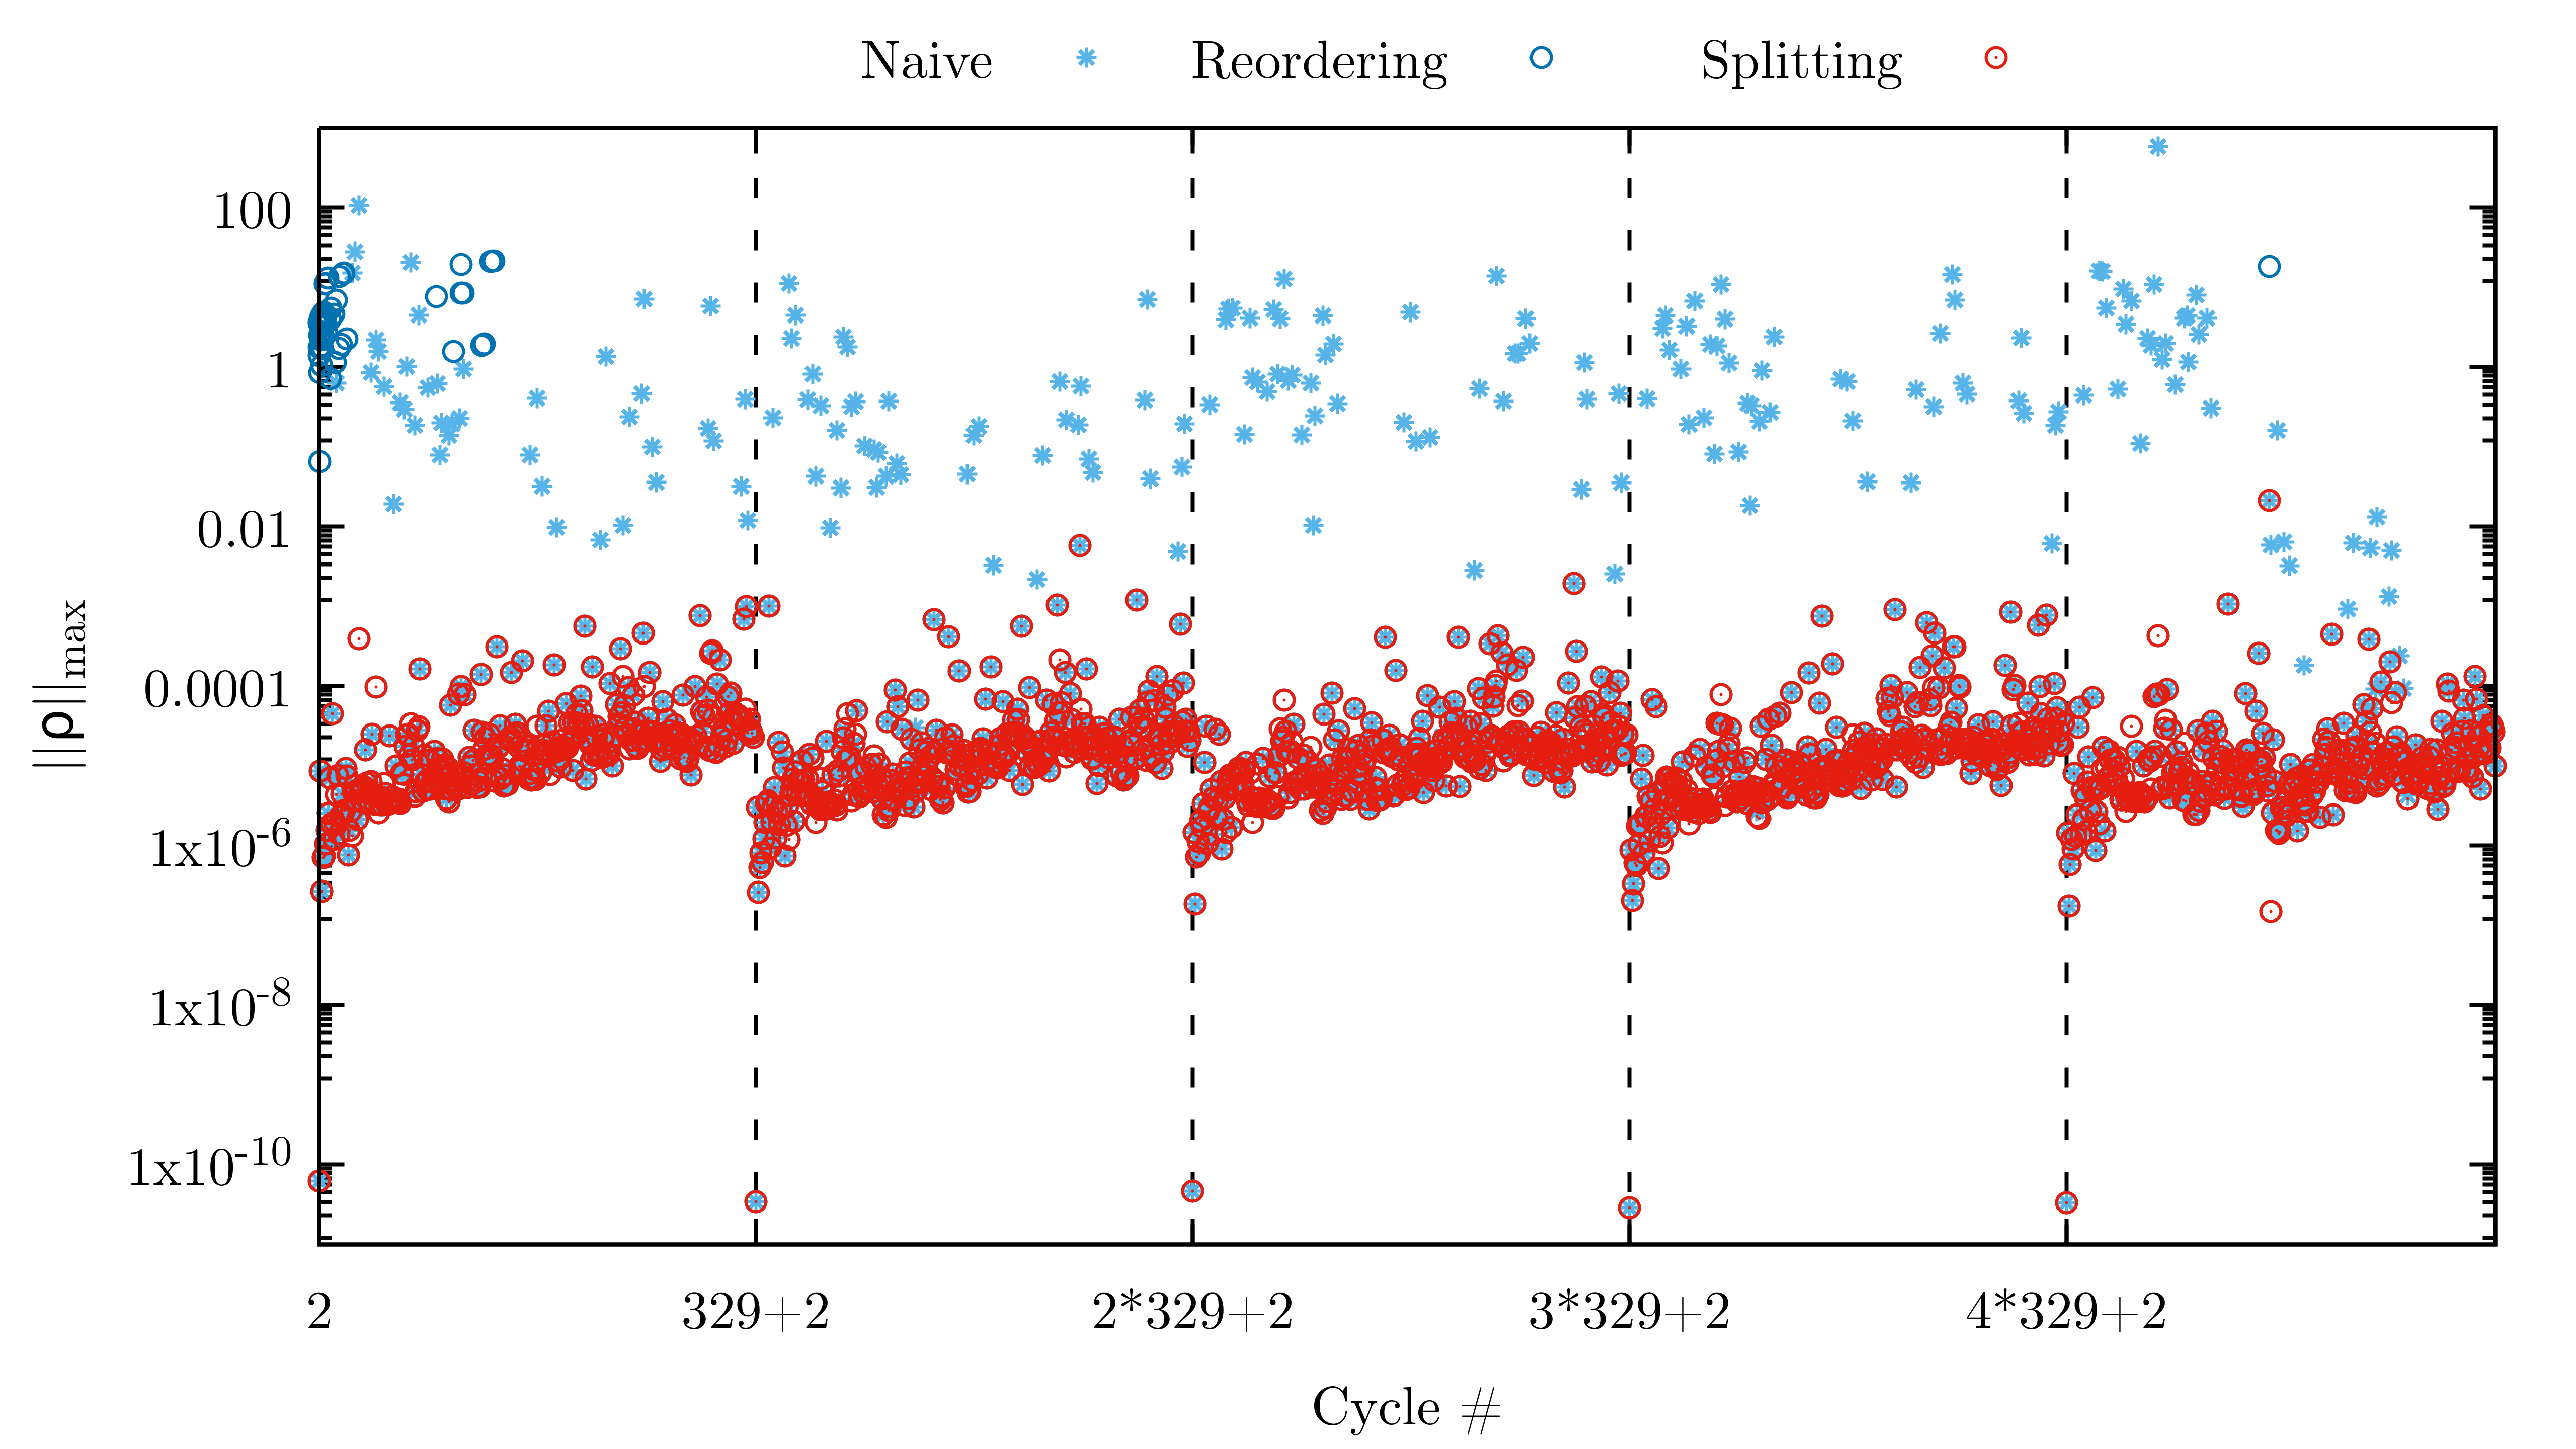
\includegraphics[width=\linewidth]{drift.png}
	\caption{Numerical drift, steadily increasing from the beginning to the end of the 329 determinant update chain.}
	\label{fig:numerical-drift}
\end{figure}
				
				\paragraph{Numerical accuracy independent of number of updates} Another interesting aspect of the SM and WB kernels is that the numerical accuracy, measured by  the Max-norm of the residual matrix $\rho$ does not seem to dependent on the number of rank-1 updates they have to apply. This is showed in Figure~\ref{fig:num_acc_nupds}. For most kernels and number of updates the Max-norm appears the be centred around $1\times10^{-5}$. There is one extra branch at 1 rank-1 update centred around $1\times10^{-11}$. These correspond to the second determinants in the chain as discussed just above.

\begin{figure}
	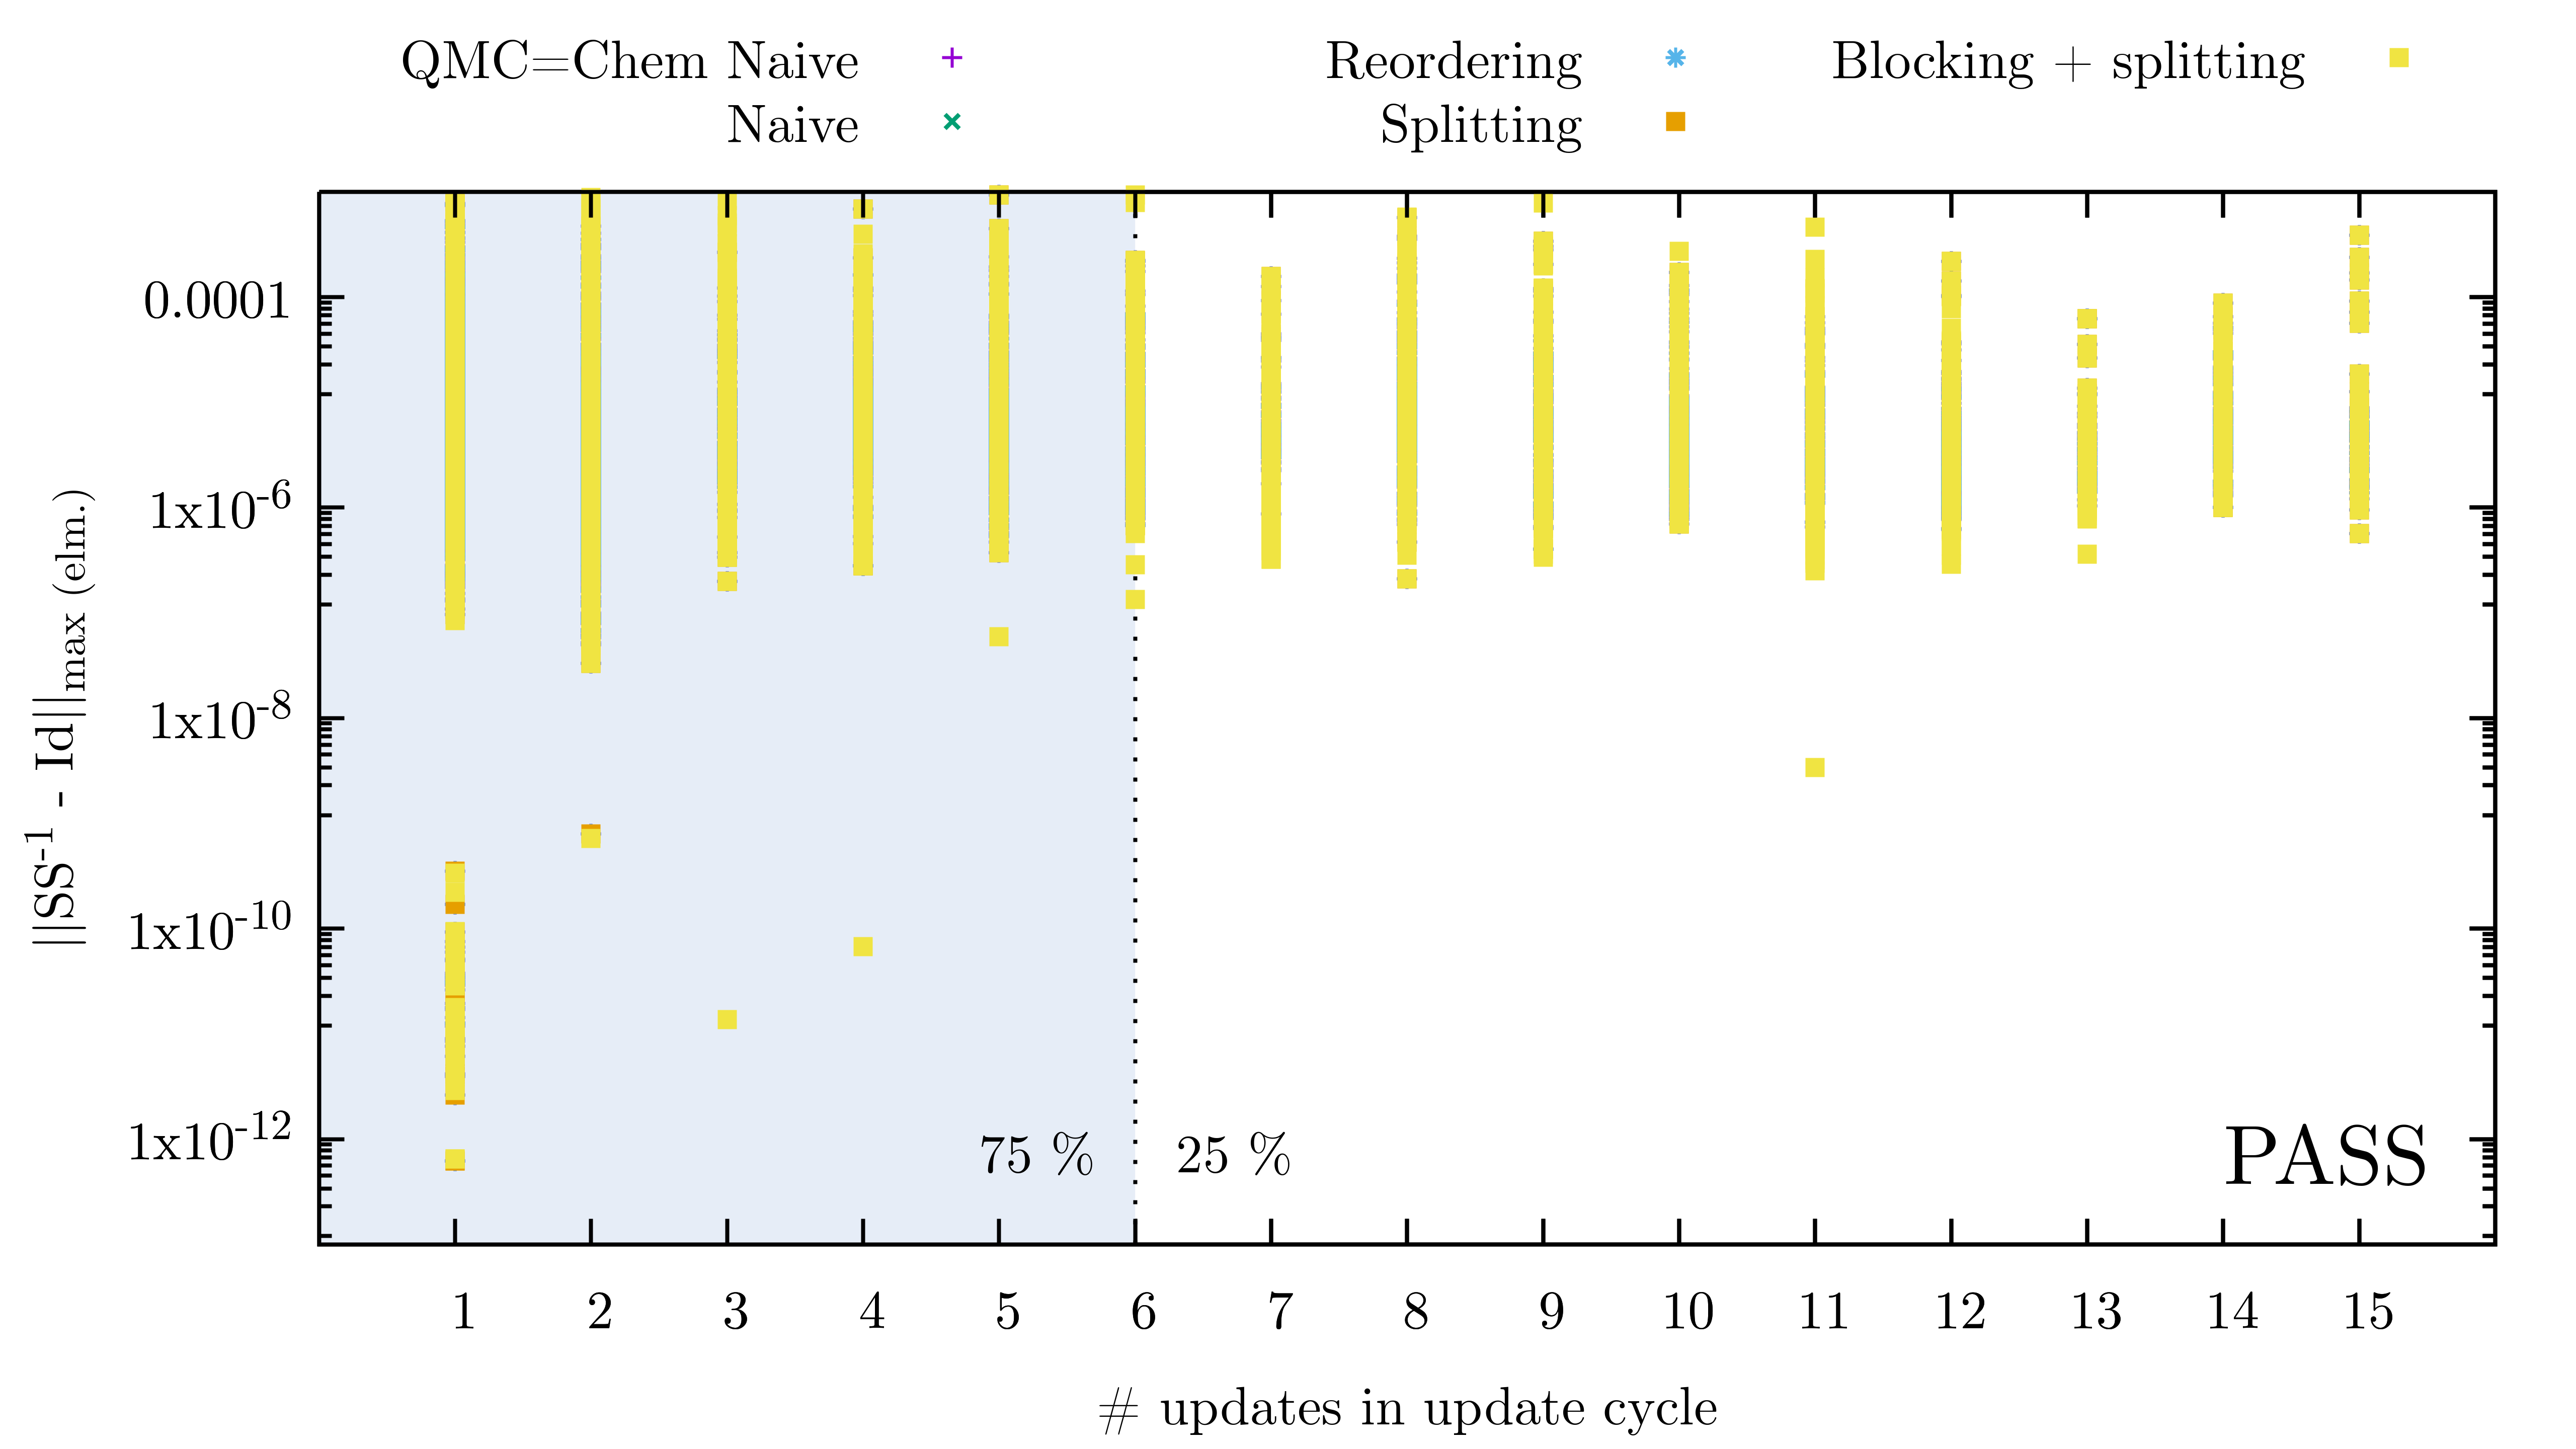
\includegraphics[width=\linewidth]{num_acc_nupds.png}
	\caption{The influence of the number of rank-1 updates to numerical accuracy for various kenrnes.}
	\label{fig:num_acc_nupds}
\end{figure}

			\subsubsection{15784 $\alpha$-determinants}
				For this case we chose to show a slightly larger level of detail by giving the fail rates for five representative number of rank-1 updates: an overall fail rate \emph{all}, the case where there is only \emph{1} rank-1 update to compare against the Na\"{i}ve kernel, \emph{2} to compare against Woodbury $2\times2$ (WB2), \emph{3} to compare against Woodbury $3\times3$ (WB3) and \emph{6} to see how well the Blocking kernel performs against Reordering/Splitting. The results are summarised in Table~\ref{tab:fr15784}. As in the 329-determinant case, the Na\"{i}ve kernel is by far the worst as rank-$k$, with $k>1$, are very common. It is surprising however that for the rank-1 update case the Na\"{i}ve kernel seems to do ever so slightly worse than the Splitting kernel, but maybe we are actually looking at the machine noise level; they are the same upto 4 decimal digits. For the rank-2 update case WB2 is slightly worse than Splitting, Reordering and Blocking because the Woodbury kernels seem cause slightly larger loss of precision than the SM-only kernels. The Blocking kernel behaves the same as the Splitting-kernel because it retries the failed cases of WB2 (because the denominator is too small) by sending them to the Splitting kernel and then passes. For WB3 we see the same behaviour for the rank-3 update cases. The failing blocks are retried using the Splitting kernel. Overall the Blocking and Splitting kernels behave numerically equivalent and are the best compared to the others. The Blocking kernel is a few more failing cases because WB2 and WB3 are slightly less accurate, but as we will see later this comes with a slight increase in speed.

	\begin{table}[h]
	\begin{tabular}{@{}l|rrrrrr@{}}
	\toprule
	\small{\#~upds~(222008 cycles)} & Kernel:~~Na\"{i}ve & Splitting & Reordering & WB2  & WB3  & Blocking \\ \midrule
	all (222008 cycles)				& 48.780			 & .831		 & .932       &	--	 & --   & .831  	   \\ \specialrule{0.1pt}{1pt}{1pt}
	1 (23533 cycles)					& .939				 & .931		 & .939       &	--   & --   & .931     \\ \specialrule{0.1pt}{1pt}{1pt}
	2 (29388 cycles)					& 5.962				 & .759		 & .769	 	  &	.783 & --   & .759     \\ \specialrule{0.1pt}{1pt}{1pt}
	3 (26239 cycles)					& 54.545			 & .808		 & .873       &	--	 & .842 & .808     \\ \specialrule{0.1pt}{1pt}{1pt}
	6 (19442 cycles)					& 73.835			 & .741		 & .905       &	--	 & --   & .746     \\ \bottomrule
	\end{tabular}
	\caption{Fail rates for Benzene with 15784 $\alpha$-determinants, 222008 determinants in total, $\beta=1\times10^{-3}$ and $\tau=1\times10^{-3}$. The fail rates are shown for five relevant number of updates.}\label{tab:fr15784}
\end{table}			
			
		\subsection{Results for the performance}
		
			\subsubsection{Performance per rank-1 update}
			
			\begin{figure}[h]
				\centering
				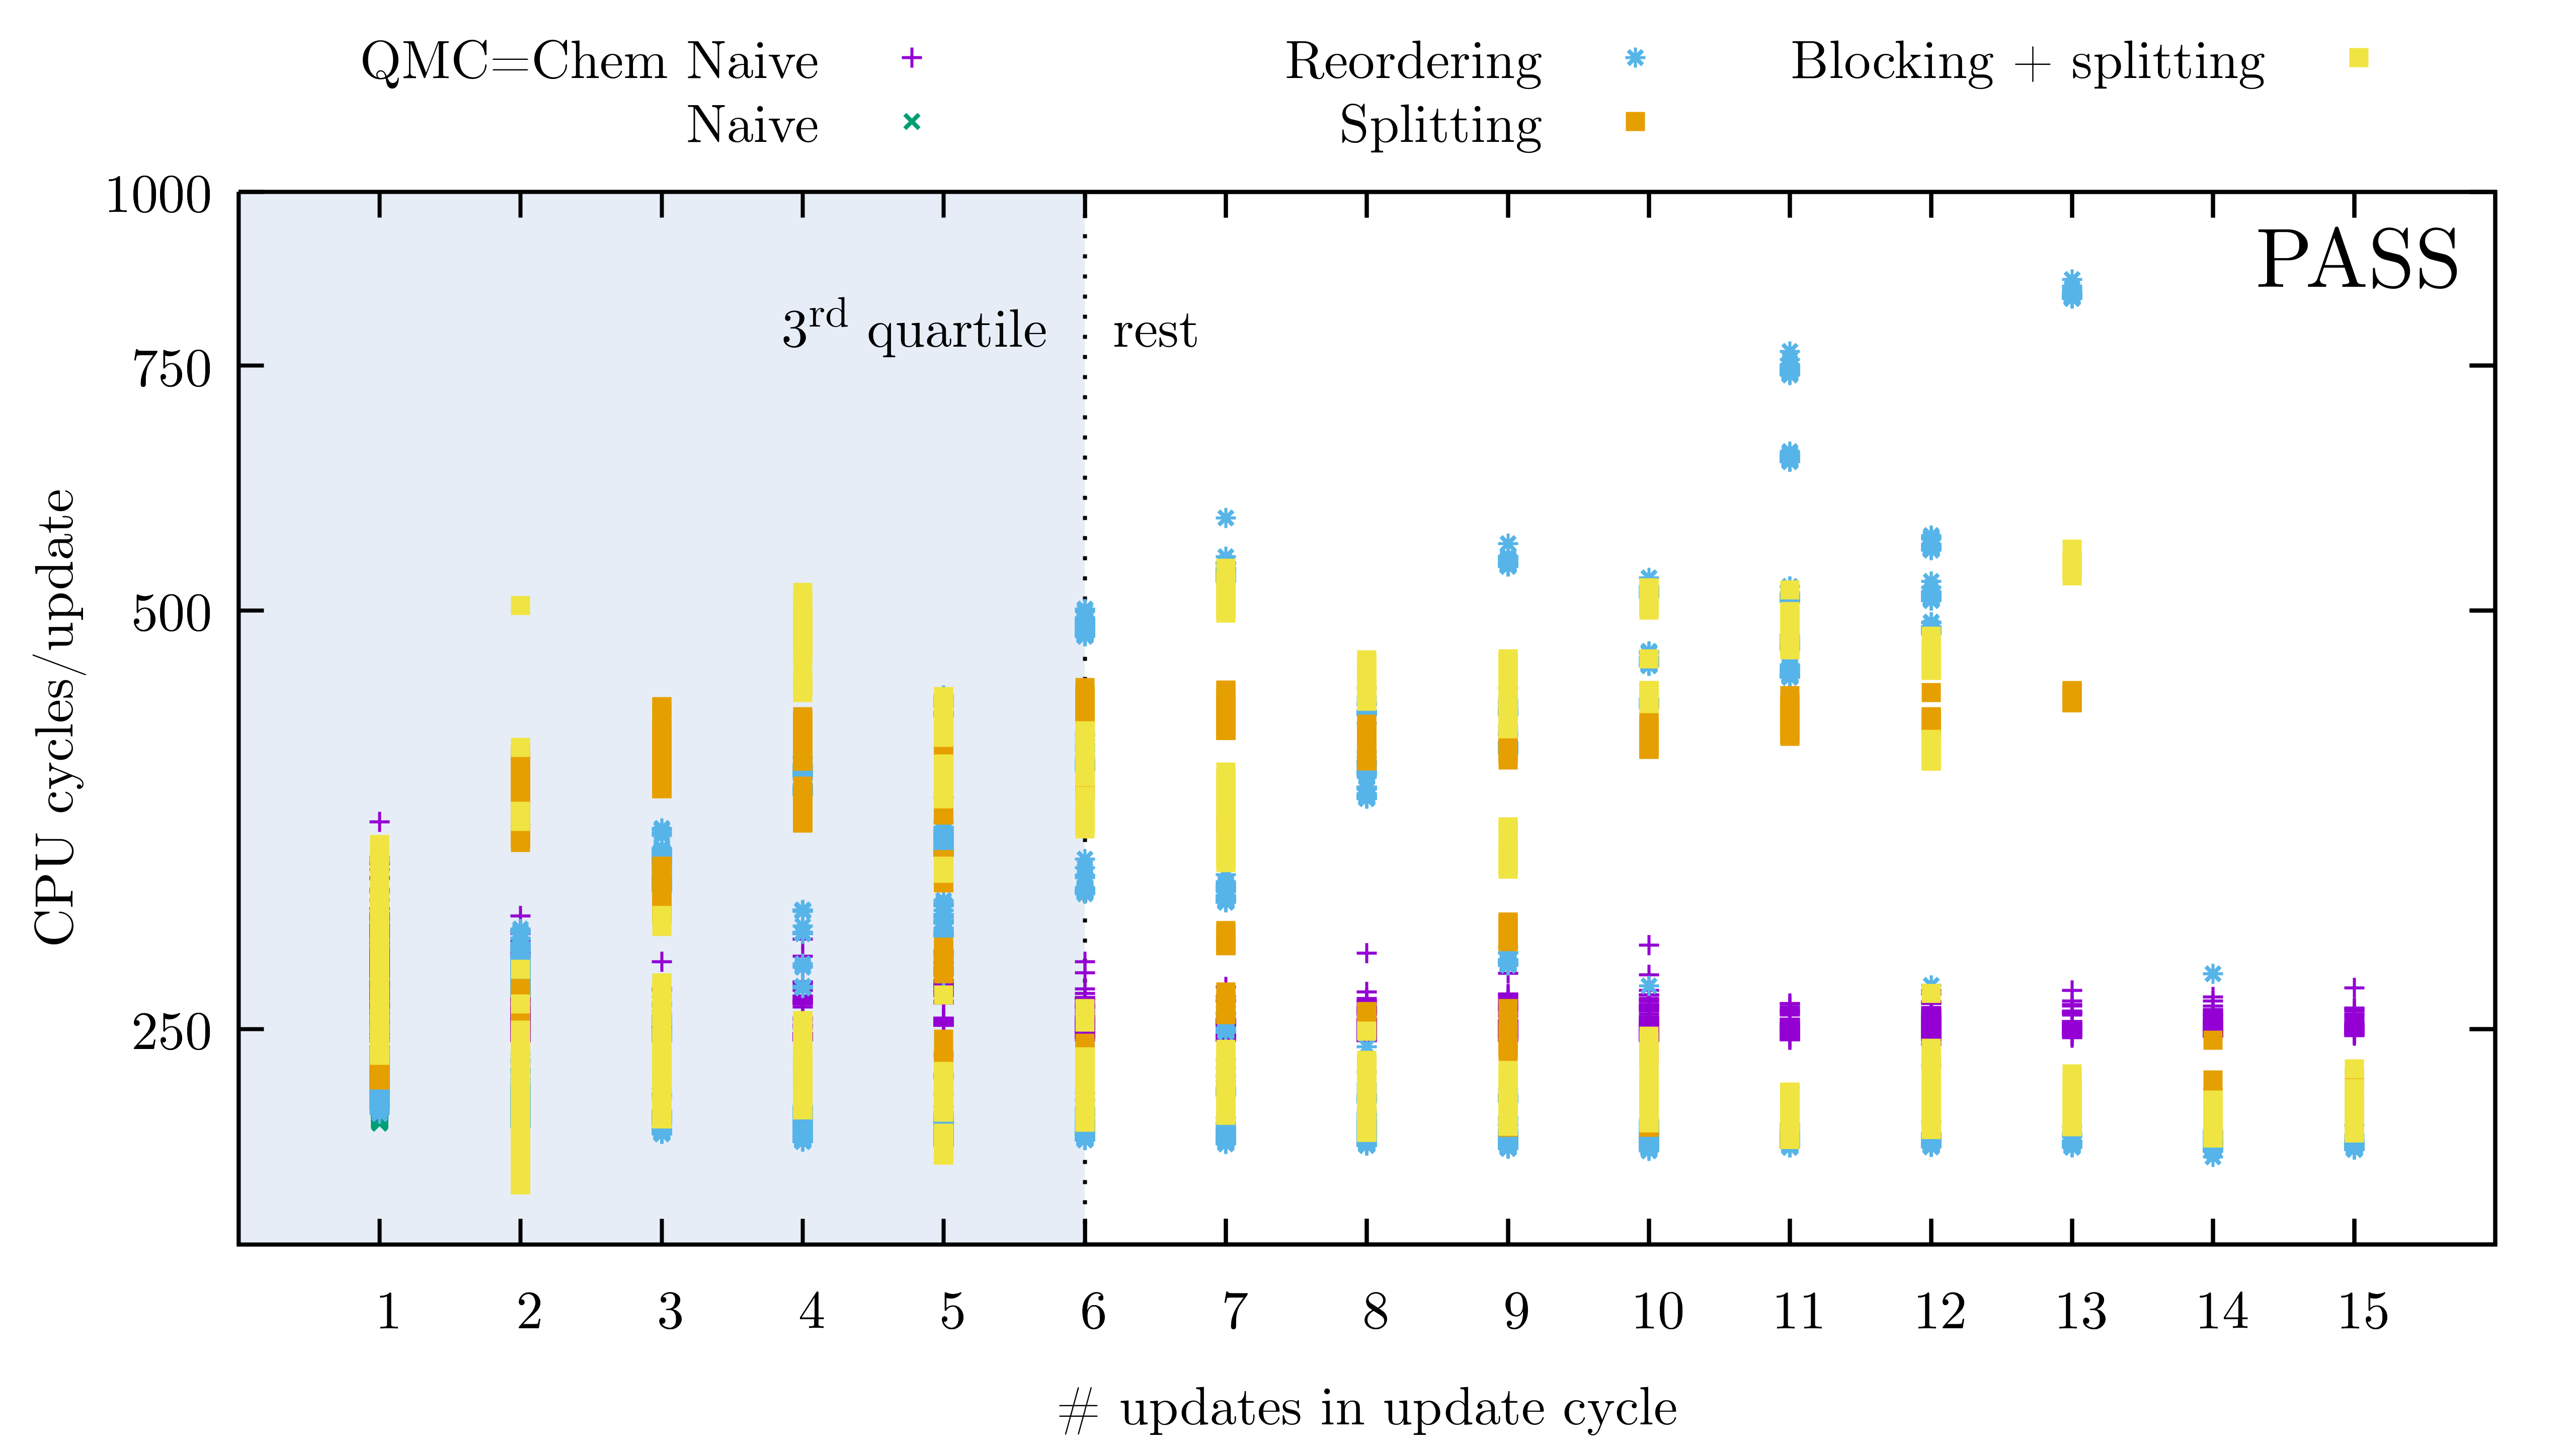
\includegraphics[width=1\textwidth]{perf_per_update.png}
				\caption{Performance in CPU-cycles per rank-1 update for various kernels.}
				\label{fig:perf_per_update}
			\end{figure}	

			In Fig.~\ref{fig:perf_per_update} is shown the number of CPU-cycles per rank-1 update versus the number of rank-1 updates for various kernels. Focussing our attention on the $3^\mathrm{rd}$ there are two main branches. One is centred around 250 CPU-cycles/rank-1 update. For one rank-1 update the spread is due to variability of the machine itself. For the cases of more than one rank-1 update this is mainly due to the number of splits for the Splitting kernel, or the number of failed blocks in the Blocking kernel.\\
							
			Looking at the left two panels of Fig.~\ref{upds_nsplits_cpucycles}, for the case of Benzene, 329 determinants the maximum number of splits is always one less than the number of updates, in case of the Splitting kernel. The Blocking kernel seems to get away with less splits in general, except in the case of two rank-1 updates. On the right two panels of Fig.~\ref{upds_nsplits_cpucycles} we plotted the average number of CPU cycles per rank-1 update as a function of the number of splits. In  the \textsc{passing} cases the number of CPU cycles per update increase linearly as the number of splits increases, up until 6 splits where it plateaus. For the \textsc{failing} cases there are never more than 3 splits, but most of these occurences are clustered around 0--2 splits and take an average of about 300 CPU cycles per update. 

			\begin{figure}[h]
				\centering
				\includegraphics[width=1\textwidth]{upds_nsplits_cpucycles.png}
				\caption{Distribution of the occurrence frequency for each number of rank-1 updates that can occur. The blue area represents the $3^\mathrm{rd}$ quartile of the distribution. For the 329-determinants case, 75\% of the time updates consist of 1--6 rank-1 updates. For the 15784-determinants case updates consist of 1--8 rank-1 updates.}
				\label{upds_nsplits_cpucycles}
			\end{figure}
						

		\subsubsection{Performance stratification}
		
		When you look at Fig.~\ref{fig:pareto_all} of everything together, all kernels, all updates, pass and fail, it you get a good overview of the whole space of possibilities but you cannot see well what is going on for each individual kernel. It is still somewhat instructive because you can see that most of the failures come from Naive and QMC=Chem Naive (covered by Naive). That was to be expected.
		\begin{figure}
			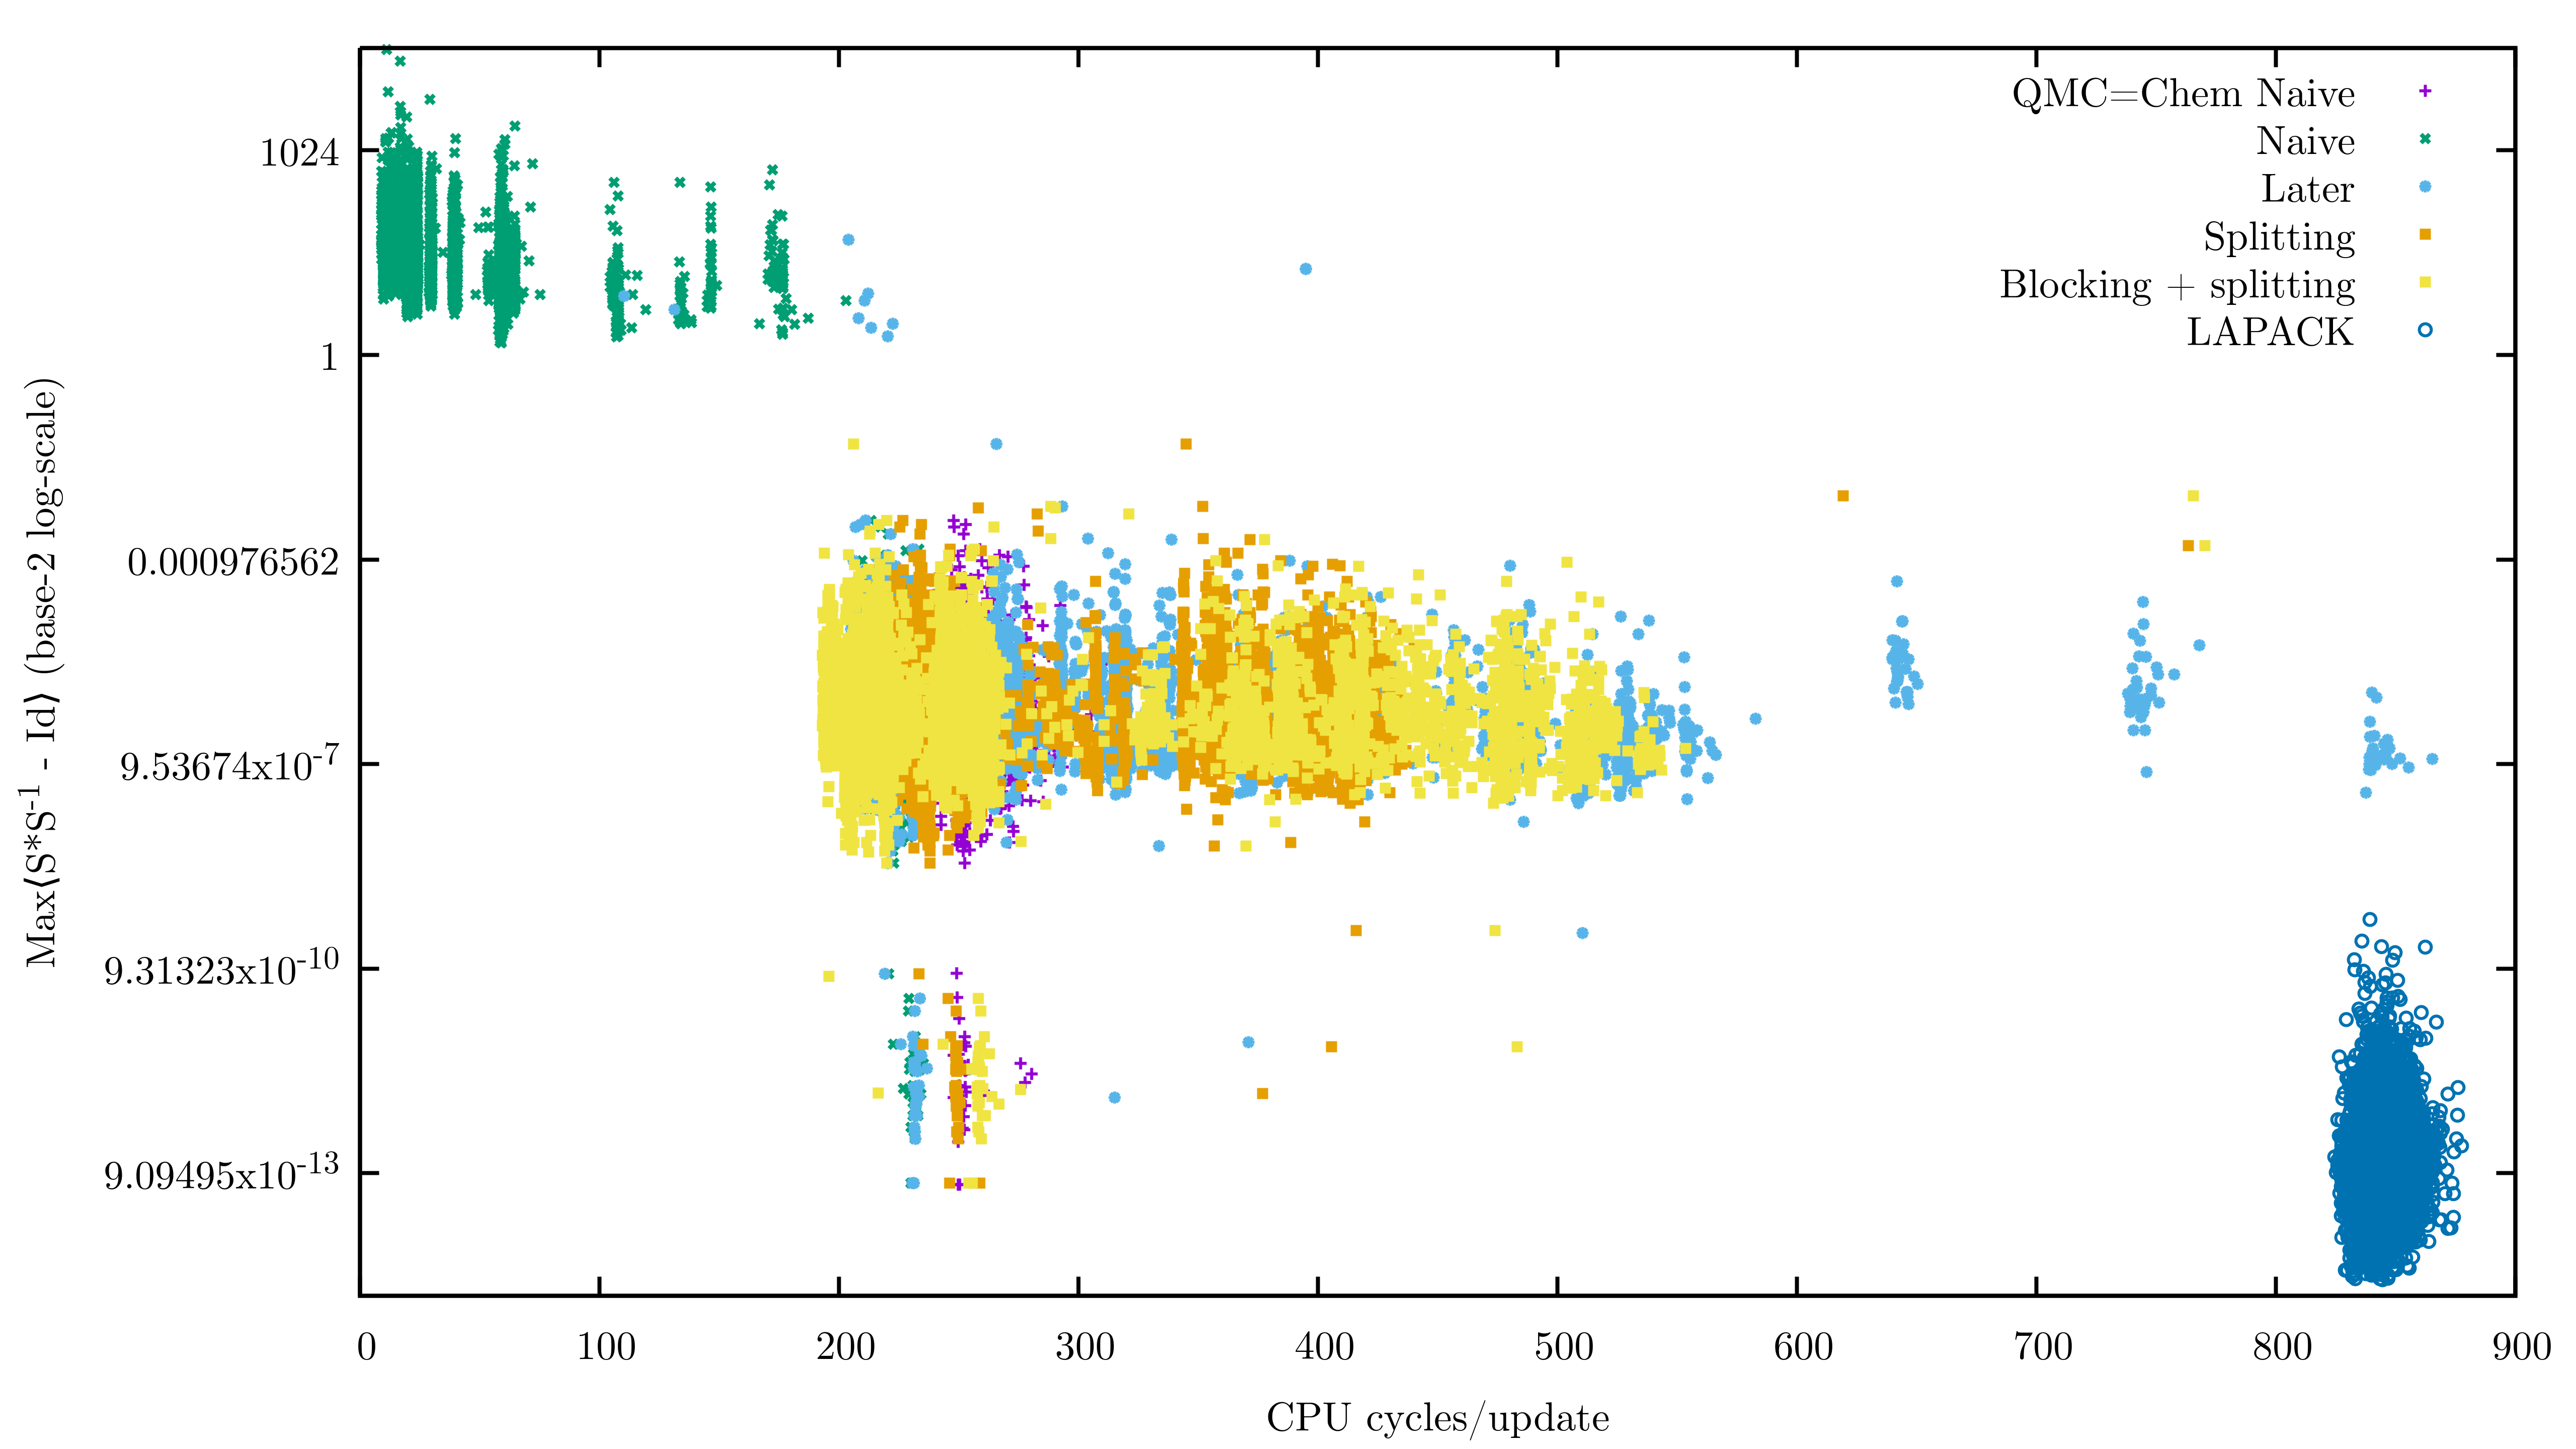
\includegraphics[width=\linewidth]{pareto_pass_fail_all.png}	
			\caption{The accuracy ($||SS^{-1}-I||_\mathrm{max}$) vs. the performance for all tested kernels, above and below the acceptance tolerance.}
			\label{fig:pareto_all}
		\end{figure}
		
2. In Fig.~\ref{fig:pareto_pass} we are only looking at the cycles that passed. It is already a bit better but is still a bit messy. Not sure this plot is much better than the first one. Maybe we should not include it.
		\begin{figure}
			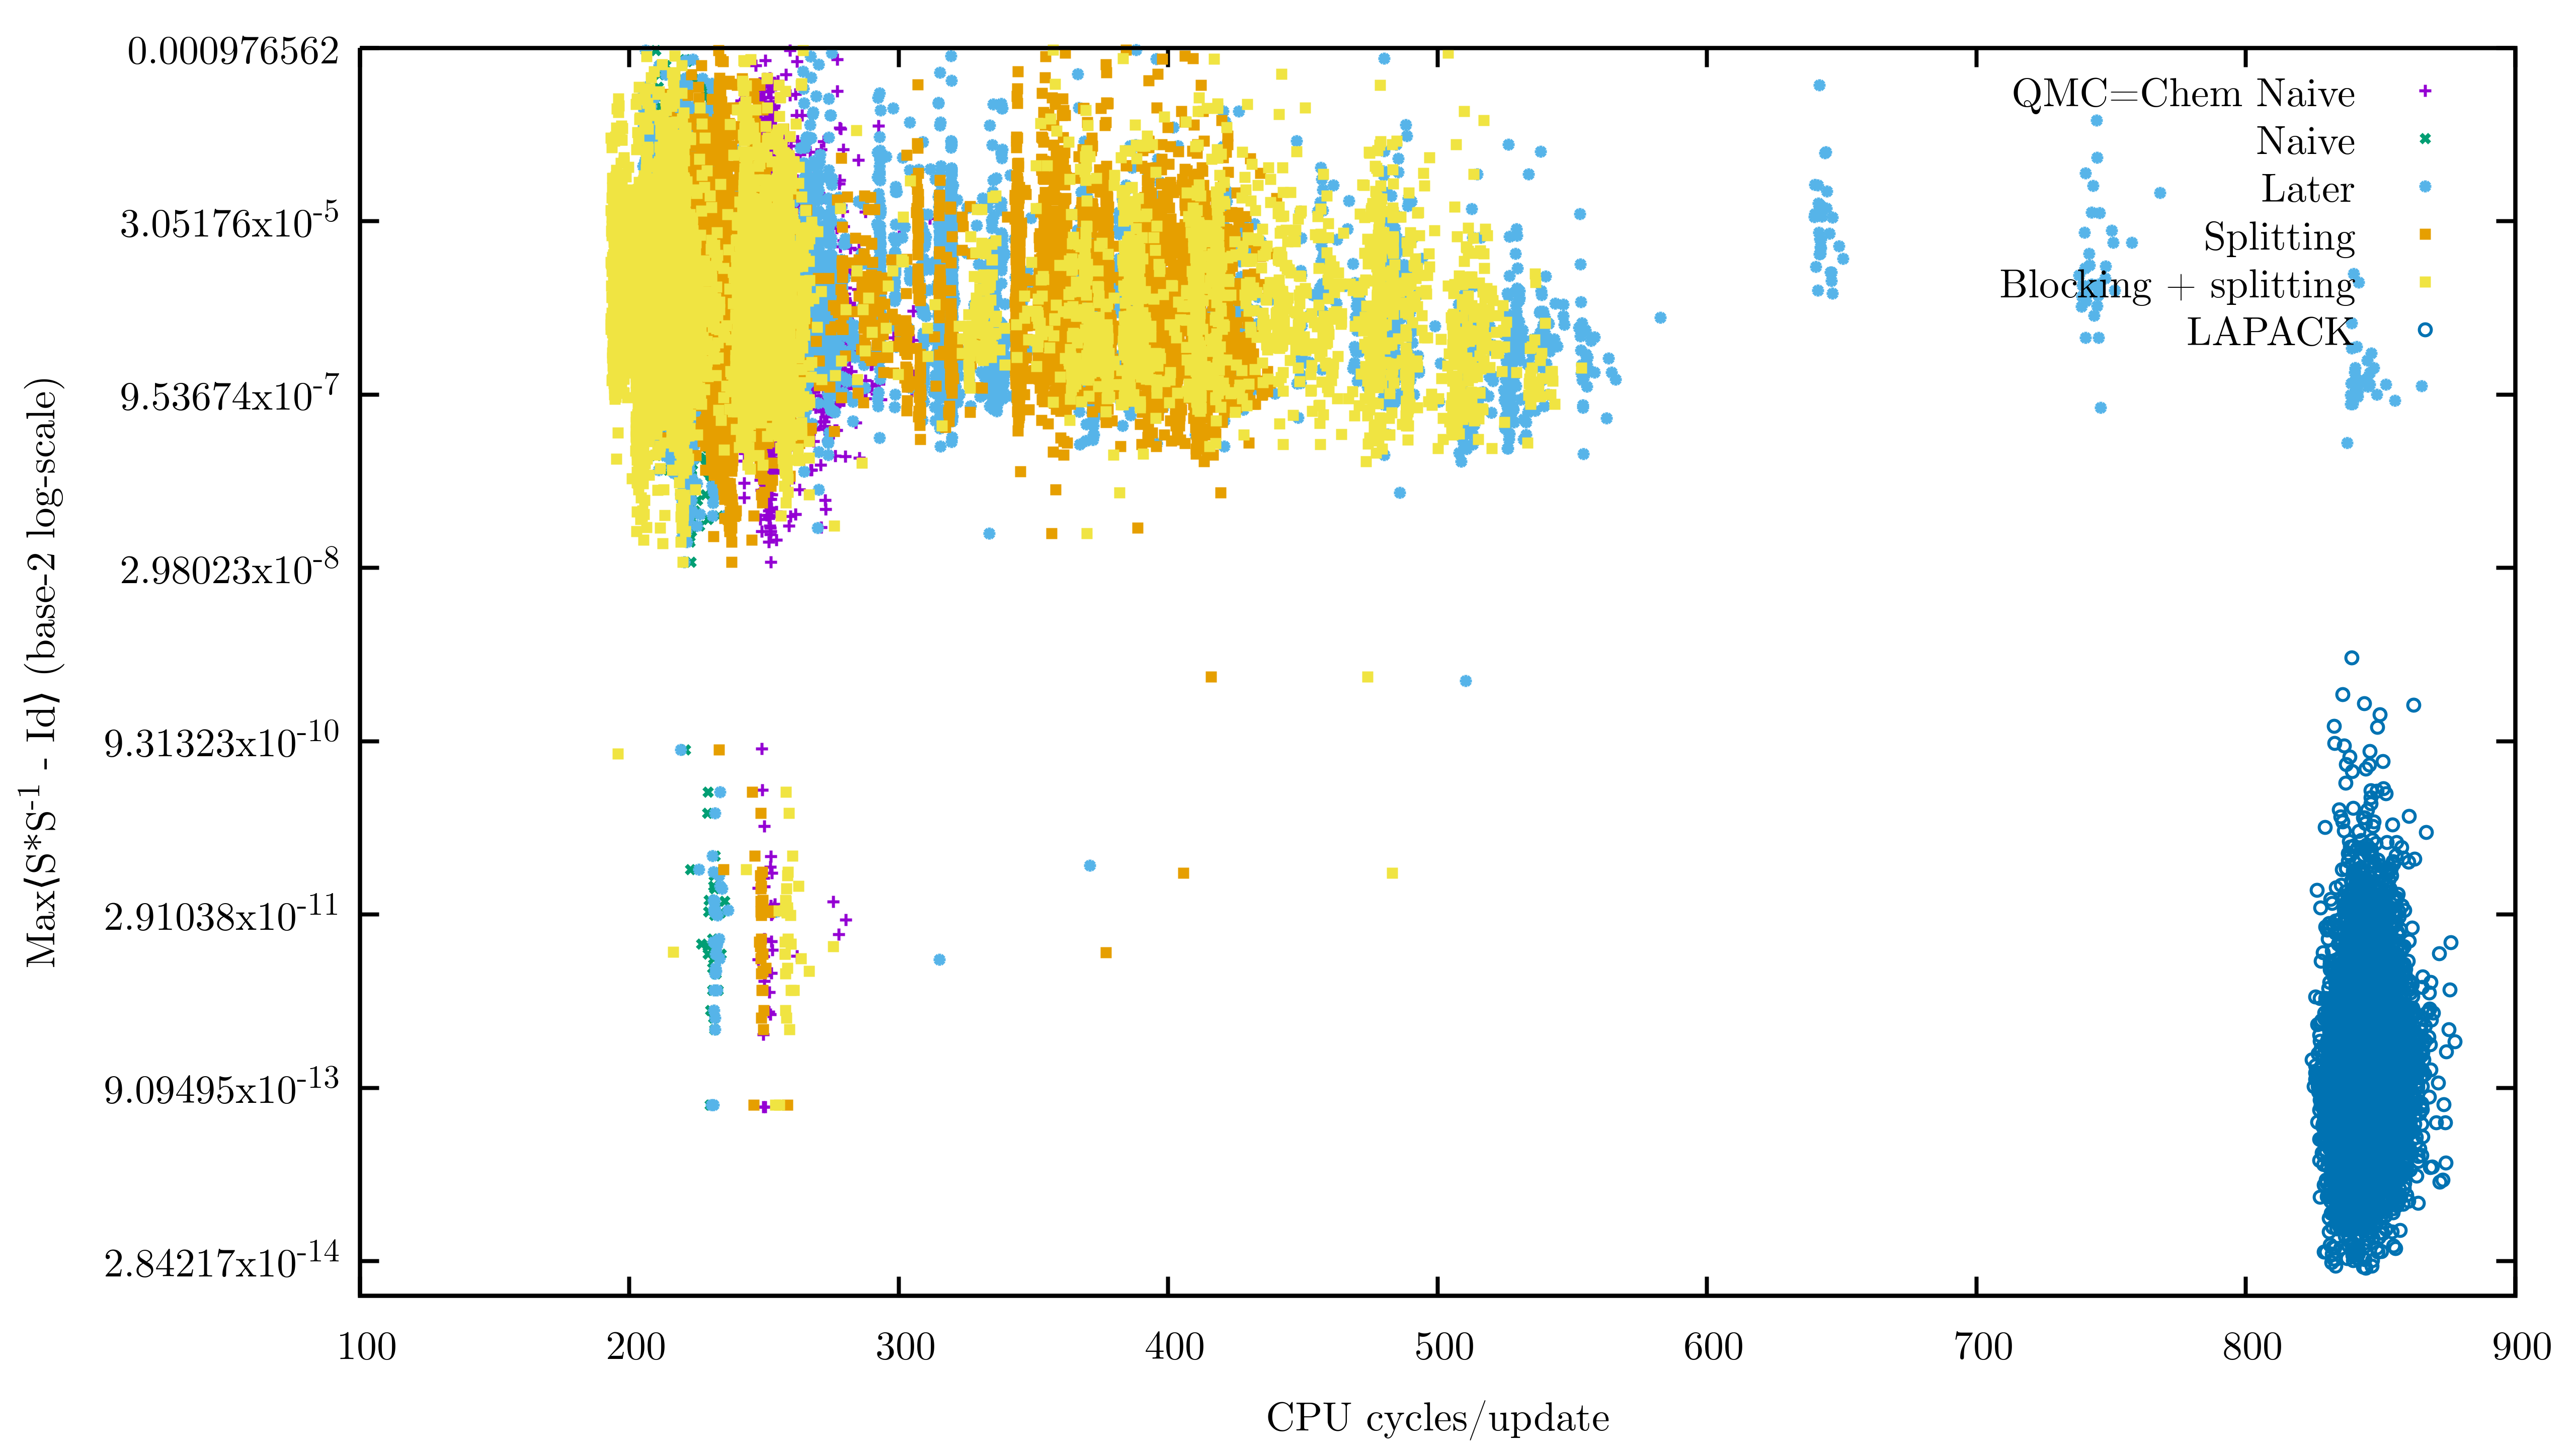
\includegraphics[width=\linewidth]{pareto_pass_all.png}	
			\caption{The accuracy ($||SS^{-1}-I||_\mathrm{max}$) vs. the performance for all tested kernels, above and below the acceptance tolerance.}
			\label{fig:pareto_pass}
		\end{figure}
3. In the third plot I focused on only the passed updates with 9 cycles. This is already much cleaner and gives a better idea of what the kernels are doing. And it is here were you can clearly see some stratification of the clusters for each individual kernel, except for the 2 Naive ones and LAPACK.

4. To understand the stratification I thought of zooming in on one kernel to see if it had something to do with splitting. So the next plot only shows the Pareto plot for all passed  9-update cycles of the splitting kernel. Here you can see clearly 4 distinct bands. First I thought this was linked to the maximum number of splits for a given 9-update cycle. But this is not the case because the maximum number of splits is 8 and there are not 9 bands (one extra for 0 splits). Then I thought it could be related to the number of recursions the kernel calls itself, but this was also not the case because the maximum number of recursions is only 1x: all splits happen in the first pass and get completed in the second pass (for 9-update cycles). Finally it is related to the number of splits, but not all number of splits happen. In fact only 0, 1, 3, 7 and 8 splits happen for 9-update cycles. So when you then split out the data for these number of splits you get the final plot.
5. In the last plot you can clearly see that the bands correspond to each bin of number of splits. There are actually 5 bands, but the band for 8-splits only contains 2 points and is very close to the points for the 7-split band. If there were more points I am sure they. would form a band as well. I am pretty convinced this also explains the bands in the performance plots for splitting 
@Eric P.
 mentioned 2 weeks ago when I was at UVSQ.
For the Later-kernel these bands must be related to the number of recursions because it doesn’t do splitting. For the Blocked kernel it is also splitting but the distribution of the number of splits is modulated by the fact some Woodbury blocks of 3 succeed where there would otherwise be a split. If it is needed I can do the same analysis for the Blocked kernel. (
			

  \section{Discussion and recommendation}
			\subsection{Final classification of all the kernels}
		
			Fig.~\ref{fig:Pareto_passfail_mean}
		
			\begin{figure}[h]
				\centering
				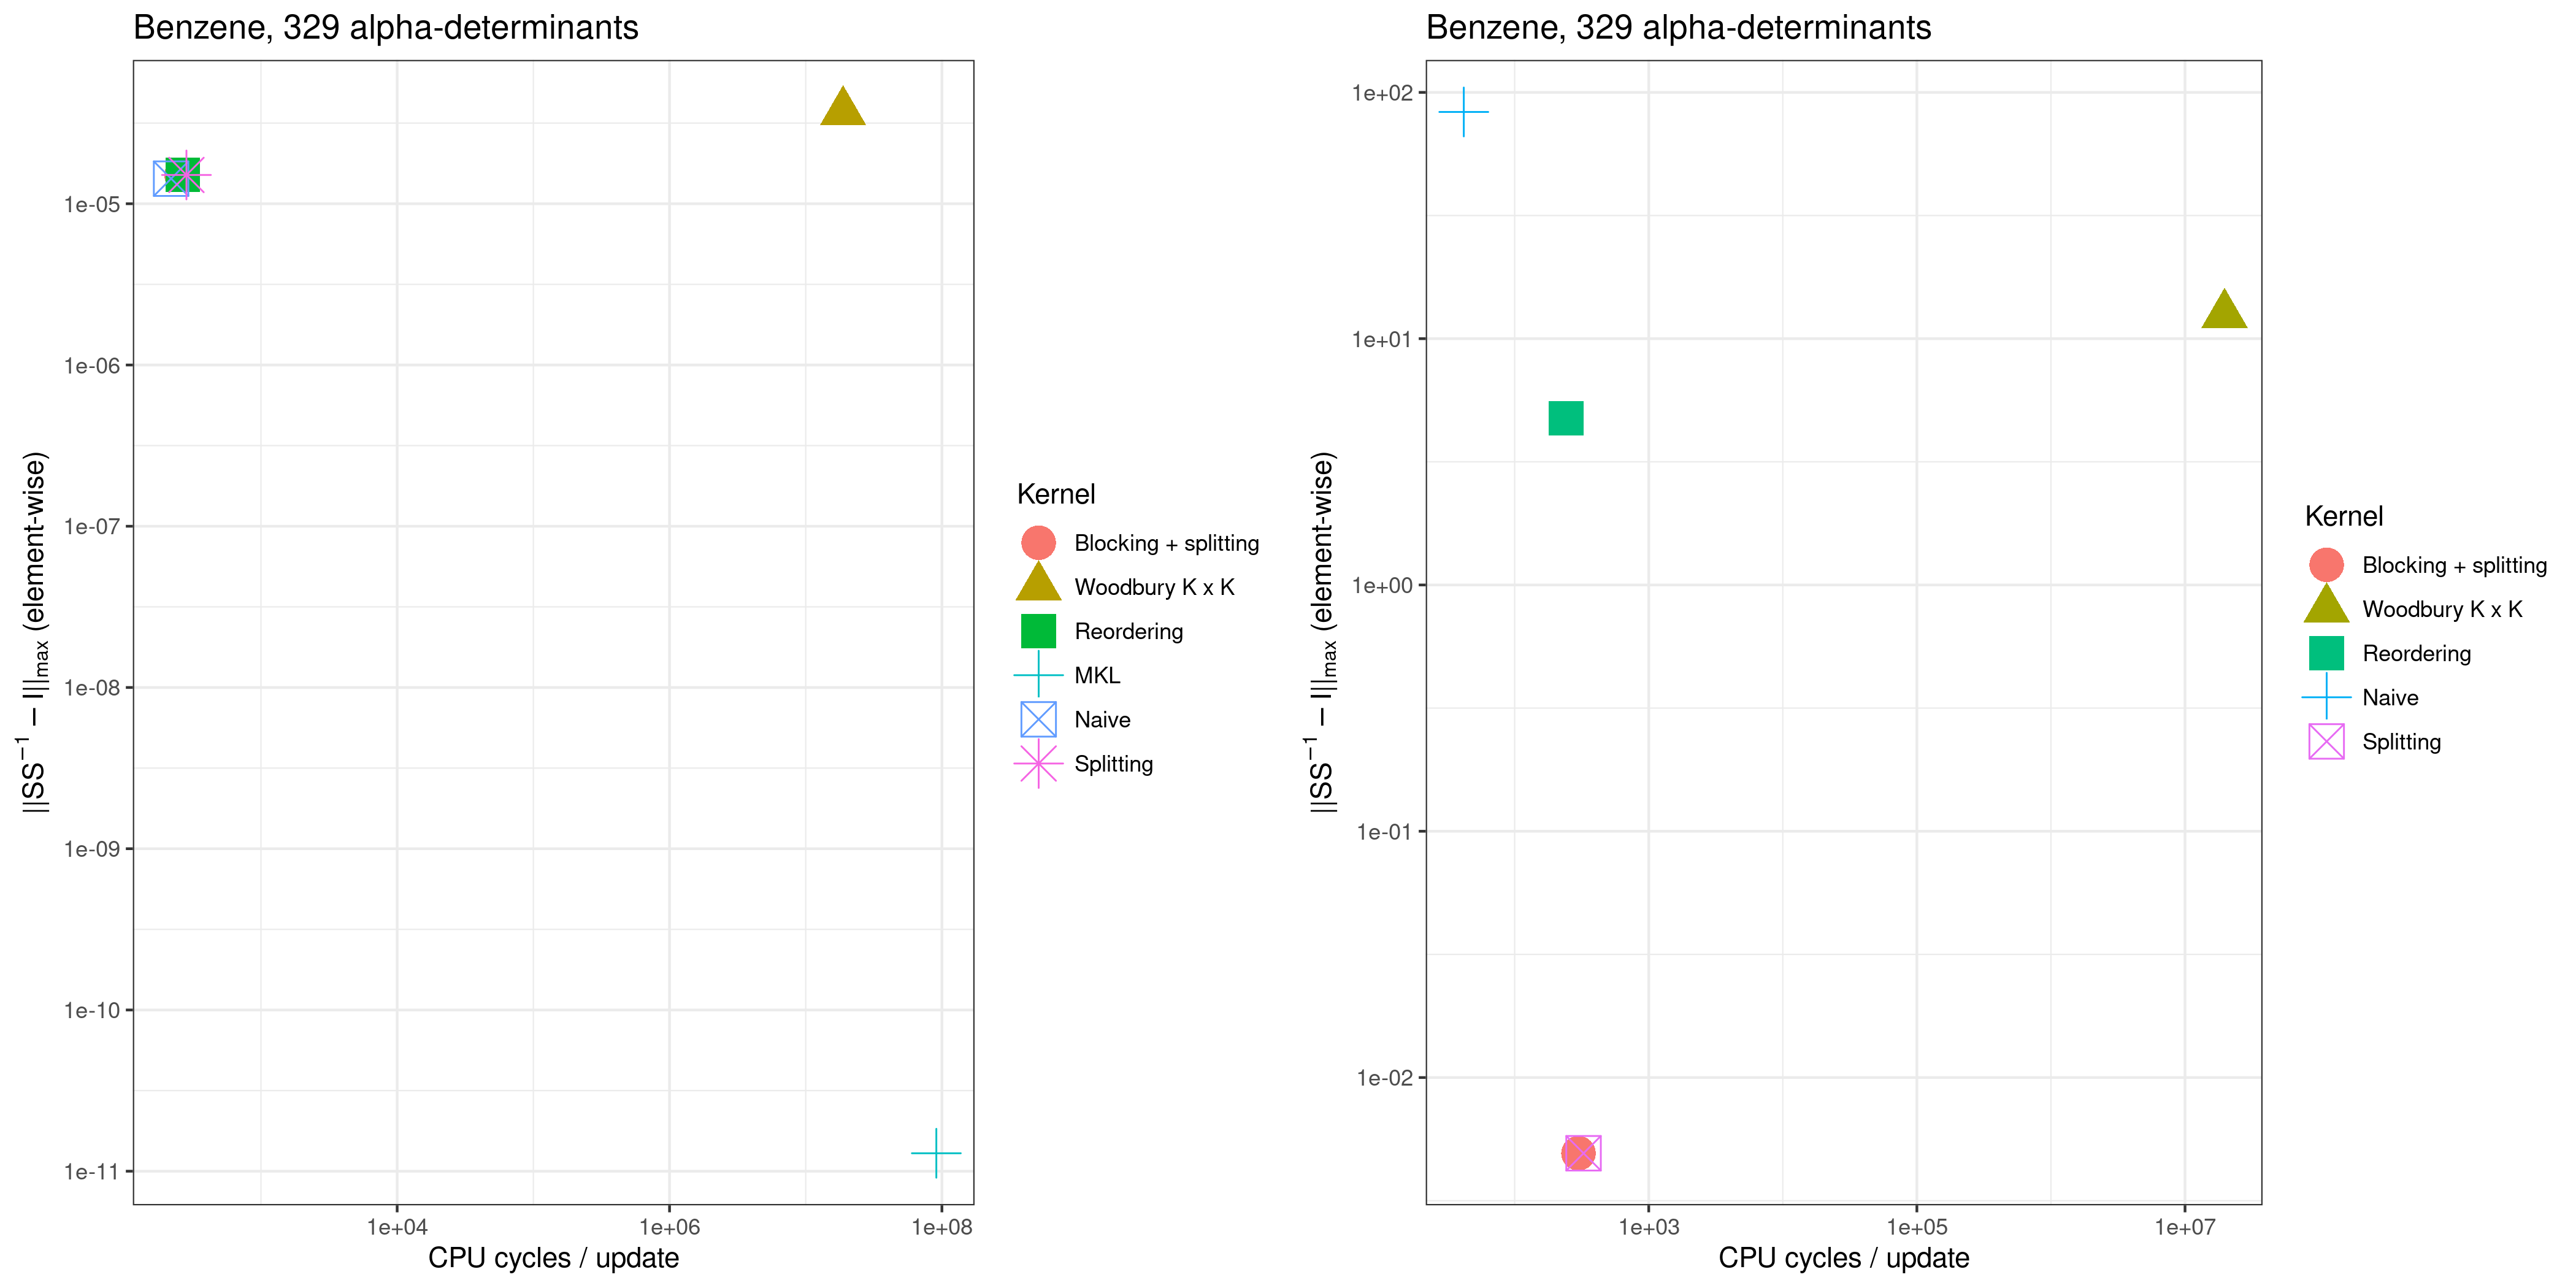
\includegraphics[width=1\textwidth]{Pareto_passfail_mean.png}
				\caption{kjkjkj}
				\label{fig:Pareto_passfail_mean}
			\end{figure}
	
  \section{Inclusion in Quantum Monte Carlo Kernel Library}
    Since this work has been funded by and executed in the context of the TREX Centre of Excellence in HPC for Quantum Chemistry, all the computational kernels that are presented in this report (except the kernel outlined in Section~3.2) are included in the TREX Centre of Excellence Quantum Monte Carlo Kernel Library (TREX-CoE/QMCkl). The repository where the QMCkl code and documentation is stored can be found on \url{https://github.com/TREX-CoE/qmckl}.\\
    
    The kernels themselves as well as the code, documentation and regression testes can be found in an `Org-mode' formatted file can be found the \texttt{org/} subdirectory at \url{https://github.com/TREX-CoE/qmckl/blob/master/org/qmckl_sherman_morrison_woodbury.org}.\\
    
    The HPC versions of these kernels can be found at \url{https://github.com/TREX-CoE/qmckl/tree/master/org/hpc}

  \newpage
  \appendix

\section{Sherman-Morrison with zero-padding}

We can now use this to add padding to the Sherman-Morrison formula to make it more efficient in SIMD enabled CPUs. We go from using matrices $S$, $S^{-1}$ and $u$ to using matrices $\widetilde{S}$, $\widetilde{S}^{-1}$ and $\widetilde{u}$
\begin{align}
	\left(S+uv^\top \right)^{-1} &= S^{-1}-\frac{S^{-1}uv^\top S^{-1}}{1+v^\top S^{-1}u} \\
								&\downarrow \\
	\left(\widetilde{S}+\widetilde{u}v^\top \right)^{-1} &= \widetilde{S}^{-1}-\frac{\widetilde{S}^{-1}\widetilde{u}v^\top \widetilde{S}^{-1}}{1+v^\top \widetilde{S}^{-1}\widetilde{u}} \\
								&\Updownarrow \\
	\left(P^\top S+P^\top uv^\top \right)^{-1} &= S^{-1}P-\frac{S^{-1}PP^\top uv^\top S^{-1}P}{1+v^\top S^{-1}PP^\top u}	
\end{align}
for padding added to the columns of $S$ and $u$ and to the rows of $S^{-1}$. This insures that
\begin{align}
	\widetilde{S}^{-1}\widetilde{S} &= S^{-1}PP^\top S \\
									&= S^{-1}IS \\
									&= S^{-1}S
\end{align}

\section{Woodbury with zero-padding}
For the Woodbury formula we proceed in the same way. The matrices $S$, $S^{-1}$ and $U$ are replaced by $\widetilde{S}$, $\widetilde{S}^{-1}$ and $\widetilde{U}$
\begin{align}
\left(S+UV\right)^{-1} &= S^{-1} - S^{-1}U(I+VS^{-1}U)^{-1}VS^{-1}\\
	&\downarrow \\
\left(\widetilde{S}+\widetilde{U}V\right)^{-1} &= \widetilde{S}^{-1} - \widetilde{S}^{-1}\widetilde{U}(I+V\widetilde{S}^{-1}\widetilde{U})^{-1}V\widetilde{S}^{-1} \\
		&\Updownarrow \\
\left(P^\top S+P^\top UV\right)^{-1} &= S^{-1}P - S^{-1}PP^\top U(I+VS^{-1}PP^\top U)^{-1}VS^{-1}P
\end{align}

\clearpage
\addcontentsline{toc}{section}{References}
\bibliographystyle{abbrv}
\bibliography{SMWB_report.bib}
		
\end{document}
